\documentclass[11pt,a4paper]{article}
\usepackage[a4paper,top=25mm,bottom=24mm,left=24mm,right=24mm,headheight=14pt]{geometry}
\usepackage{fontspec}
\IfFontExistsTF{Times New Roman}{\setmainfont{Times New Roman}}{\setmainfont{TeX Gyre Termes}}
\usepackage{amsmath,amssymb,mathtools,bm}
\usepackage{graphicx}
\usepackage{booktabs,tabularx,array}
\usepackage{caption}
\usepackage{float}
\usepackage{indentfirst} 
\usepackage{xcolor}
\usepackage{enumitem}
\usepackage{fancyhdr}
\usepackage{titlesec}
\usepackage{hyperref}
\usepackage{xurl}
\usepackage{listings}
\usepackage{fancyvrb}
\newfontfamily\treefont{DejaVu Sans Mono}

\DefineVerbatimEnvironment{filetree}{Verbatim}{
  formatcom=\treefont\small,
  xleftmargin=1em
}

\emergencystretch=2em
\setlength{\parindent}{2em}

\definecolor{deepnavy}{HTML}{16385C}
\definecolor{marsred}{HTML}{A64235}
\hypersetup{colorlinks=true,linkcolor=deepnavy,citecolor=marsred,urlcolor=deepnavy}
\graphicspath{{../figures/}}
\captionsetup{font=small,labelfont={bf,color=deepnavy},labelsep=space}
\setlist{nosep,leftmargin=1.8em}
\titleformat{\section}{\Large\bfseries\color{deepnavy}}{\thesection}{0.7em}{}
\titleformat{\subsection}{\large\bfseries\color{deepnavy}}{\thesubsection}{0.6em}{}
\titleformat{\subsubsection}{\normalsize\bfseries\color{marsred}}{}{0pt}{}
\pagestyle{fancy}
\fancyhf{}
\fancyhead[L]{\small Going to Mars: Keplerian Orbits and Real Transfers}
\fancyhead[R]{\small\thepage}

\newcommand{\vect}[1]{\bm{#1}}
\newcommand{\norm}[1]{\left\lVert#1\right\rVert}
\newcommand{\kms}{\ensuremath{\,\mathrm{km\,s^{-1}}}}
\newcommand{\AU}{\ensuremath{\,\mathrm{AU}}}
\makeatletter
\newcommand{\vinf}{\@ifnextchar_{\vinf@sub}{v_{\infty}}}
\def\vinf@sub_#1{v_{\infty,#1}}
\makeatother
\newcommand{\code}[1]{\texttt{#1}}
% Single source of cover-page metadata. Edit here before final submission.
\newcommand{\CourseName}{MATH2850J Honors Mathematics III}
\newcommand{\ProjectName}{Going to Mars: From Conic Geometry to Transfer Design}
\newcommand{\InstructorName}{Professor Horst Hohberger}
\newcommand{\GroupName}{Group 19}
\newcommand{\SubmissionDate}{11 July 2026}
\newcommand{\AuthorList}{%
Kemeng Lu\\
Chenming Tao\\
Peikai Mao\\
Zhuo Chen\\
Website: \url{https://kimonlu.github.io/MATH2850J-Project-Going-to-Mars-Web/}\\
Repository: \url{https://github.com/KimonLu/MATH2850J-Project-Going-to-Mars-Web}}


\newcommand{\HohmannTOF}{258.9}
\newcommand{\HohmannDVOne}{2.945}
\newcommand{\HohmannDVTwo}{2.649}
\newcommand{\HohmannEarthSpeed}{29.785}
\newcommand{\HohmannMarsSpeed}{24.129}
\newcommand{\HohmannTransferDepartureSpeed}{32.729}
\newcommand{\HohmannTransferArrivalSpeed}{21.480}
\newcommand{\HohmannDepartureEnergy}{92.046}
\newcommand{\HohmannArrivalEnergy}{60.409}
\newcommand{\HohmannTransferEnergy}{-351.517}
\newcommand{\HohmannCThree}{8.672}
\newcommand{\HohmannLEODV}{3.611}
\newcommand{\HohmannLMODV}{2.096}
\newcommand{\HohmannPhase}{44.35}
\newcommand{\HohmannSynodic}{779.9}
\newcommand{\HohmannPatchedDV}{5.708}
\newcommand{\MinimumDeparture}{2026-11-01 06:00}
\newcommand{\MinimumArrival}{2027-09-07 12:00}
\newcommand{\MinimumTOF}{310.25}
\newcommand{\MinimumCThree}{9.27}
\newcommand{\MinimumArrivalVInf}{2.568}
\newcommand{\MinimumLEODV}{3.638}
\newcommand{\MinimumLMODV}{2.058}
\newcommand{\MinimumTotalDV}{5.696}
\newcommand{\MinimumTransferAngle}{204.76}
\newcommand{\MinimumTransferInclination}{1.05}
\newcommand{\MinimumTransferSemimajor}{1.269}
\newcommand{\MinCThreeDeparture}{2026-10-31 12:00}
\newcommand{\MinCThreeArrival}{2027-08-19 18:00}
\newcommand{\MinCThreeTOF}{292.25}
\newcommand{\MinCThreeCThree}{9.18}
\newcommand{\MinCThreeArrivalVInf}{2.72}
\newcommand{\MinCThreeTotalDV}{5.763}
\newcommand{\CircularMinimumDeparture}{2026-12-06}
\newcommand{\CircularMinimumArrival}{2027-08-21}
\newcommand{\CircularMinimumTOF}{258.0}
\newcommand{\CircularMinimumCThree}{8.68}
\newcommand{\CircularMinimumArrivalVInf}{2.65}
\newcommand{\CircularMinimumTotalDV}{5.708}
\newcommand{\StandishMinimumDeparture}{2026-10-31 06:00}
\newcommand{\StandishMinimumArrival}{2027-09-07 06:00}
\newcommand{\StandishMinimumTOF}{311.00}
\newcommand{\StandishMinimumCThree}{9.23}
\newcommand{\StandishMinimumTotalDV}{5.695}
\newcommand{\RealMinusCircularDV}{-0.012}
\newcommand{\RealMinusCircularTOF}{52.2}
\newcommand{\RealMinusStandishDV}{0.0004}
\newcommand{\RealMinusStandishDepartureDays}{1.00}
\newcommand{\RealMinusStandishTOF}{-0.75}
\newcommand{\FastDeparture}{2026-11-18}
\newcommand{\FastArrival}{2027-07-28}
\newcommand{\BalancedDeparture}{2026-12-06}
\newcommand{\BalancedArrival}{2027-06-26}
\newcommand{\FastCThree}{12.68}
\newcommand{\FastArrivalVInf}{3.21}
\newcommand{\BalancedCThree}{23.04}
\newcommand{\BalancedArrivalVInf}{4.52}
\newcommand{\BalancedTOF}{202.0}
\newcommand{\BalancedTotalDV}{7.427}
\newcommand{\FastTOF}{252.0}
\newcommand{\FastTotalDV}{6.172}
\newcommand{\ActualDVPenaltyPercent}{-0.21}
\newcommand{\ActualTOFPenaltyPercent}{19.85}
\newcommand{\FastDVPenaltyPercent}{8.37}
\newcommand{\BalancedDVPenaltyPercent}{30.40}
\newcommand{\LambertEndpointError}{0.001191}
\newcommand{\CThreeStabilityWorstPenalty}{0.60}
\newcommand{\TotalDVStabilityWorstPenalty}{0.037}
\newcommand{\StandishEarthMedianPositionError}{2149}
\newcommand{\StandishEarthMaximumPositionError}{10947}
\newcommand{\StandishEarthMedianVelocityError}{0.48}
\newcommand{\StandishEarthMaximumVelocityError}{1.65}
\newcommand{\StandishMarsMedianPositionError}{37494}
\newcommand{\StandishMarsMaximumPositionError}{61187}
\newcommand{\StandishMarsMedianVelocityError}{3.15}
\newcommand{\StandishMarsMaximumVelocityError}{5.25}
\newcommand{\OberthGainRatio}{5.31}
\newcommand{\SolarGM}{132712440041.279388}


\begin{document}

\begin{titlepage}\centering
{\Large \CourseName\par}\vspace{1.6cm}
{\Huge\bfseries \ProjectName\par}\vspace{0.45cm}
{\Large A complete mathematical modelling report\par}\vfill
\begin{tabular}{rl}Instructor: & \InstructorName\\ Group: & \GroupName\\ Submitted: & \SubmissionDate\end{tabular}
\vfill {\large \AuthorList\par}
\end{titlepage}
\begin{abstract}
This report develops a unified mathematical framework for Earth--Mars trajectory design, progressing from Keplerian orbit geometry to date-specific interplanetary transfers and gravity-assisted extensions. We derive the conic classification of two-body trajectories, the geometric relations of elliptical orbits, the orbital-energy identity, and the vis-viva equation. These results are used to construct an analytic Hohmann-transfer benchmark before the circular, coplanar assumptions are replaced by DE440s planetary states and a universal-variable Lambert solver for the 2026--2027 launch opportunity. Porkchop maps, local stability tests, and Pareto analysis are then used to compare launch energy, total patched-conic impulse, and flight time. Finally, planet-centred hyperbolic geometry is used to explain how gravity assists extend the feasible design space of multi-leg missions. The report links analytic derivations, numerical results, and reproducibility information within a single model hierarchy.
\end{abstract}
\tableofcontents\newpage

\section{Introduction and Research Objectives}
\label{sec:introduction}

Interplanetary trajectory design is naturally organized as a hierarchy of
models. Keplerian two-body mechanics provides the geometric and energetic
structure of an orbit; the Hohmann transfer supplies an analytic benchmark for
motion between idealized circular orbits; an ephemeris-driven Lambert solution
then determines date-specific transfer arcs; and gravity-assist analysis
extends the same framework to multi-leg missions.

The report refines this hierarchy by comparing two distinct ephemeris
representations: the high-fidelity NASA/JPL DE440s integrated numerical
ephemeris and the computationally efficient secular Keplerian approximation
based on the Standish--Williams elements (JPL-approx). This comparison,
carried out across the 2026--2027 launch opportunity, isolates the impact of
higher-order gravitational perturbations and allows for a quantitative
assessment of the model-dependent shifts in the predicted launch windows.

Real-world mission design heavily relies on data-driven validation. The
practical outputs of this numerical campaign include porkchop maps for launch
energy and velocity impulses, Pareto trade-off frontiers between flight time
and fuel consumption, and stability contour plots near the optimal candidates.
Additionally, the theoretical framework is validated through numerical
reconstructions of canonical historical gravity assists, such as the Voyager 1
Jupiter encounter and the Cassini Venus-Venus-Earth-Jupiter gravity-assist
chain, using actual DE440s planetary states. By processing real NASA/JPL
planetary states into executable mission metrics, the report bridges abstract
orbital mechanics with practical, reproducible mission design.

The objectives of this report are:
\begin{enumerate}
  \item to derive the mathematical relations that connect central-force motion,
        conic sections, orbital energy, and the vis-viva equation;
  \item to obtain a symbolic Earth--Mars Hohmann transfer and interpret its
        velocity, time, and energy requirements as an ideal benchmark;
  \item to evaluate the 2026--2027 Earth--Mars launch opportunity using
        planetary ephemerides, Lambert solutions, porkchop maps, and
        multi-objective mission metrics;
  \item to examine how planet-centred hyperbolic encounters can modify
        interplanetary trajectories and support multi-leg mission design.
\end{enumerate}

The report therefore moves from exact analytic results to increasingly realistic
numerical models. Each later stage retains the insight of the preceding model
while making explicit the assumptions required for practical trajectory
selection.

\section{Keplerian Foundations}
\label{sec:keplerian-foundations}

\subsection{Why a central inverse-square force produces conics}

With the Sun treated as the dominant gravitating body, the spacecraft obeys the
two-body equation
\begin{equation}
  \ddot{\vect r}=-\frac{\mu}{r^3}\vect r,\qquad \mu=GM.
  \label{eq:twobody}
\end{equation}
The force is radial, so the specific angular momentum
$\vect h=\vect r\times\vect v$ is conserved and the motion remains in a fixed
plane. Setting $u=1/r$ and using the true anomaly $\theta$ as the independent
variable gives Binet's equation,
\begin{equation}
  \frac{d^2u}{d\theta^2}+u=\frac{\mu}{h^2}.
\end{equation}
Hence the orbit is a conic with the attracting body at one focus:
\begin{equation}
  r(\theta)=\frac{p}{1+e\cos(\theta-\theta_0)},\qquad
  p=\frac{h^2}{\mu}.
  \label{eq:conic}
\end{equation}
The eccentricity $e$ classifies the path: $0\le e<1$ gives an ellipse,
$e=1$ gives a parabola, and $e>1$ gives a hyperbola. The same classification
is visible from the energy relation
\begin{equation}
  e^2=1+\frac{2\varepsilon h^2}{\mu^2},
\end{equation}
where bound ellipses have negative specific mechanical energy
$\varepsilon$.

\begin{figure}[H]
  \centering
  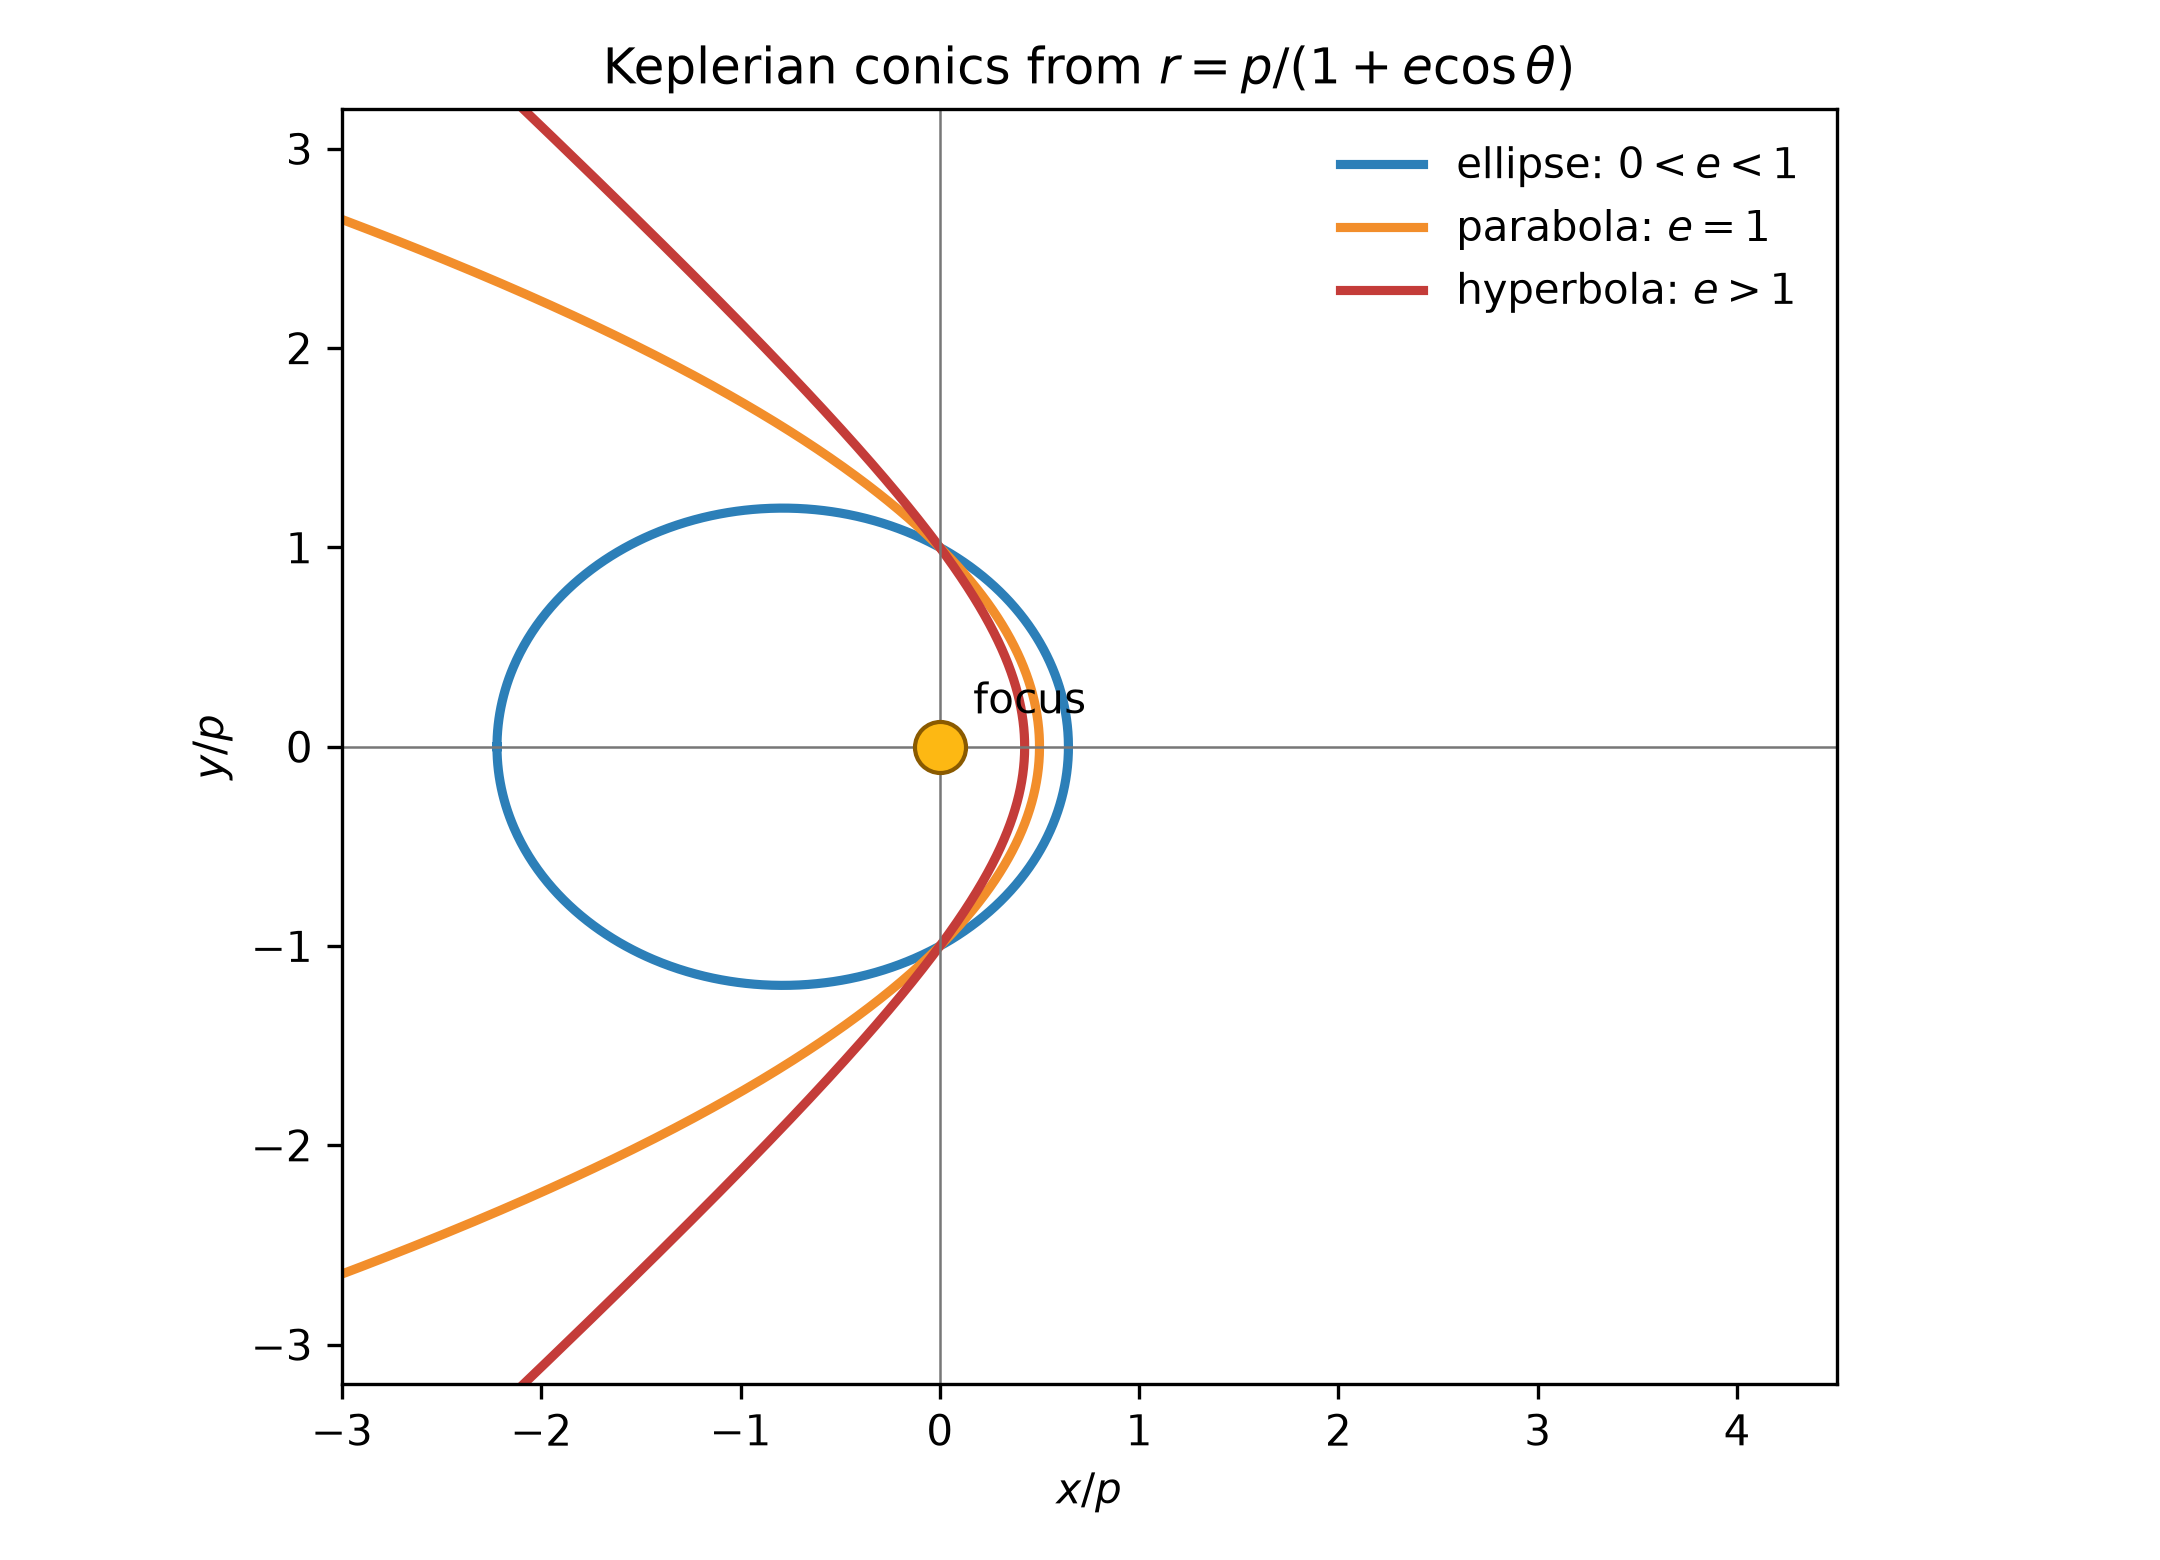
\includegraphics[width=0.76\textwidth]{keplerian_orbit_classes.png}
  \caption{Conic-section orbit classes generated by a central inverse-square force.}
  \label{fig:conics}
\end{figure}

\subsection{Ellipse geometry and the semi-minor axis}

For an ellipse, the semi-major axis is $a$, the semi-minor axis is $b$, and the
focal distance is $c=ae$. The elementary ellipse identity
\begin{equation}
  b^2=a^2-c^2
\end{equation}
therefore gives
\begin{equation}
  b=a\sqrt{1-e^2}.
  \label{eq:minor-axis}
\end{equation}
This result is not a separate dynamical law. It is the geometric consequence of
the same eccentricity that appears in the gravitational orbit equation.

\subsection{Energy conservation and the vis-viva equation}

The specific mechanical energy is
\begin{equation}
  \varepsilon=\frac{v^2}{2}-\frac{\mu}{r}.
  \label{eq:specific-energy}
\end{equation}
To rigorously derive the orbital energy relation, we evaluate this expression at periapsis and apoapsis. Let the periapsis radius and apoapsis radius be \(r_p\) and \(r_a\). From the ellipse geometry established in Section~\ref{sec:keplerian-foundations}, these are expressed as
\begin{equation}
  r_p=a(1-e), \qquad r_a=a(1+e).
\end{equation}
The spacecraft obeys angular-momentum conservation, which gives
\begin{equation}
  r_p v_p = r_a v_a.
\end{equation}
Furthermore, conservation of mechanical energy along the orbit yields
\begin{equation}
  \frac{v_p^2}{2} - \frac{\mu}{r_p} = \frac{v_a^2}{2} - \frac{\mu}{r_a}.
\end{equation}
From the angular-momentum relation we have \(v_a = v_p \frac{r_p}{r_a}\). Substituting this into the energy equation gives
\begin{equation}
  v_p^2 = \frac{2\mu r_a}{r_p(r_p+r_a)}.
\end{equation}
Substituting \(r_p=a(1-e)\) and \(r_a=a(1+e)\) yields \(r_p+r_a=2a\) and thus
\begin{equation}
  v_p^2 = \frac{\mu(1+e)}{a(1-e)}.
\end{equation}
Finally, substituting this speed and the periapsis radius back into the specific mechanical energy (Eq.~\eqref{eq:specific-energy}) gives
\begin{equation}
  \varepsilon = \frac{v_p^2}{2} - \frac{\mu}{r_p}
  = \frac{\mu(1+e)}{2a(1-e)} - \frac{\mu}{a(1-e)}
  = -\frac{\mu}{2a}.
\end{equation}
Multiplying by the spacecraft mass gives
\begin{equation}
  E=-\frac{GMm}{2a}.
\end{equation}
Substituting the specific energy back into Eq.~\eqref{eq:specific-energy} produces the vis-viva equation,
\begin{equation}
  v^2=\mu\left(\frac{2}{r}-\frac{1}{a}\right).
  \label{eq:visviva}
\end{equation}
It is the bridge between the geometric orbit size and the speed required at a given radius.

The same geometric parameters also determine the orbital period. For a closed elliptical orbit, the area swept per unit time is given by the specific angular momentum as \(\dot{A} = h/2\). Since \(h = \sqrt{\mu a(1-e^2)}\), and the total area of an ellipse is \(A = \pi a b = \pi a^2 \sqrt{1-e^2}\), the orbital period \(T\) follows as
\begin{equation}
  T = \frac{A}{\dot{A}} = \frac{\pi a^2 \sqrt{1-e^2}}{\frac{1}{2}\sqrt{\mu a(1-e^2)}} = 2\pi\sqrt{\frac{a^3}{\mu}}.
  \label{eq:kepler-third-law}
\end{equation}
This relation, which is the mathematical expression of Kepler's third law, explicitly connects the semi-major axis to the orbital period. It will be used in Section~\ref{sec:hohmann-benchmark} to calculate the symbolic flight time of the Hohmann transfer ellipse.

For the Mars-transfer problem, this equation supplies the ideal Hohmann benchmark and a useful scale for the Lambert results that follow.

\section{The Hohmann Transfer as an Analytic Benchmark}
\label{sec:hohmann-benchmark}

\subsection{Model Assumptions and Data Sources}
To simplify the trajectory analysis, the Sun is assumed to be the dominant
central body with gravitational parameter $\mu_\odot=GM_\odot$, while the
spacecraft mass is considered negligible compared with that of the Sun.
Furthermore, both the Earth and Mars are assumed to move in perfectly
circular, coplanar heliocentric orbits with radii $r_E$ and $r_M$
($r_M>r_E$), neglecting orbital eccentricity and inclination.

The orbital transfer is modelled using the impulsive-burn approximation,
where each manoeuvre is represented by an instantaneous change in velocity.
Under these assumptions, the transfer trajectory is taken to be the
classical Hohmann transfer orbit, namely an elliptical orbit tangent to
Earth's orbit at perihelion and Mars' orbit at aphelion.

According to data from NASA Jet Propulsion Laboratory (JPL) Solar System Dynamics (SSD) Group's standard parameters\cite{jplAstroPar}, the heliocentric gravitational constant (solar mass parameter) is:
\begin{equation}
    \mu_{\odot} = G M_{\odot} = 1.32712440041 \times 10^{11} \, \text{km}^3/\text{s}^2
\end{equation}

The ideal circular orbital radius of the Earth is defined as exactly $1.0 \, \text{AU}$ (Astronomical Unit). In accordance with the International Astronomical Union (IAU) 2012 Resolution B2, this baseline distance is fixed at:
\begin{equation}
    r_E = 1.0 \, \text{AU} = 149,597,870.7 \, \text{km}
\end{equation}
For Mars, the idealized circular orbit radius is anchored to its mean heliocentric semi-major axis provided by the JPL planetary satellite physical parameters database:
\begin{equation}
    r_M = 1.523662 \, \text{AU} \approx 2.27939186 \times 10^8 \, \text{km}
\end{equation}

These fundamental constants form the geometric and dynamic foundation for the analytical calculations of impulse velocity increments ($\Delta v$) and the single-trip flight time ($t_{\text{trans}}$) derived below.

\subsection{Geometry of the Hohmann Transfer Ellipse}
From the ellipse geometry developed in Section~\ref{sec:keplerian-foundations} and visualised in Figure~\ref{fig:hohmann_geo}, the semi-major axis equals the average of the perihelion and aphelion distances:
\[
a_t=\frac{r_E+r_M}{2}.
\]
This geometric parameter substitutes directly into the vis-viva equation for all speed calculations along the transfer path.

\subsection{Vis-Viva Derivation of Impulse Velocity Changes}
\subsubsection{Circular Orbit Baseline Velocity}
For any circular orbit $a=r$, substitute into vis-viva:
\[
v_c=\sqrt{\frac{\mu_\odot}{r}} \implies v_{c,E}=\sqrt{\frac{\mu_\odot}{r_E}},\quad v_{c,M}=\sqrt{\frac{\mu_\odot}{r_M}},
\]
where $v_{c,E},v_{c,M}$ are circular orbital speeds of Earth and Mars respectively.
\subsubsection{First Impulse: Earth Departure $\Delta v_1$}
At perihelion $r=r_E$, transfer ellipse speed at perihelion via vis-viva:
\[
v_{t,p}=\sqrt{\mu_\odot\left(\frac{2}{r_E}-\frac{1}{a_t}\right)}.
\]
Substitute $a_t=\dfrac{r_E+r_M}{2}$ and simplify:
\[
v_{t,p}=\sqrt{\frac{2\mu_\odot r_M}{r_E(r_E+r_M)}}.
\]
The spacecraft accelerates to leave Earth’s circular orbit, so the velocity increment is
\[
\Delta v_1=v_{t,p}-v_{c,E}=\sqrt{\frac{\mu_\odot}{r_E}}\left(\sqrt{\frac{2r_M}{r_E+r_M}}-1\right)=2.94\, \text{km/s}.
\]

\subsubsection{Second Impulse: Mars Orbit Insertion $\Delta v_2$}
At aphelion $r=r_M$, transfer ellipse speed and aphelion via vis-viva:
\[
v_{t,a}=\sqrt{\mu_\odot\left(\frac{2}{r_M}-\frac{1}{a_t}\right)}=\sqrt{\frac{2\mu_\odot r_E}{r_M(r_E+r_M)}}.
\]
The spacecraft requires a second acceleration to match Mars’ circular speed:
\[
\Delta v_2=v_{c,M}-v_{t,a}=\sqrt{\frac{\mu_\odot}{r_M}}\left(1-\sqrt{\frac{2r_E}{r_E+r_M}}\right)=2.65\, \text{km/s}.
\]

\subsubsection{Total Velocity Budget}
Total impulse requirement for the full transfer:
\[
\Delta v_{\text{total}}=\Delta v_1+\Delta v_2=5.59\, \text{km/s}.
\]
This quantity acts as the primary benchmark for relative propellant and energy consumption.

\subsection{Symbolic Transfer Flight Time Calculation}
Kepler's third law applied to the transfer ellipse gives:
\[
T^2=\frac{4\pi^2}{\mu_\odot}a^3.
\]
Full period of the Hohmann ellipse:
\[
T_t=2\pi\sqrt{\frac{a_t^3}{\mu_\odot}}.
\]
The spacecraft traverses only half the ellipse from Earth to Mars, so one-way flight time:
\[
t_{\text{trans}}=\frac{T_t}{2}=\pi\sqrt{\frac{a_t^3}{\mu_\odot}}=\pi\sqrt{\frac{(r_E+r_M)^3}{8\mu_\odot}}=258.9 \, \text{days}.
\]

\subsection{Orbital Energy Requirement}
Using the orbital-energy identity derived in Section~\ref{sec:keplerian-foundations}:
\[
E=-\frac{m\mu_\odot}{2a}.
\]
\begin{itemize}
    \item Earth circular orbit energy: $E_1=-\dfrac{m\mu_\odot}{2r_E}$
    \item Mars circular orbit energy: $E_2=-\dfrac{m\mu_\odot}{2r_M}$
\end{itemize}
Total energy increase supplied by engine burns:
\[
\Delta E=E_2-E_1=\frac{m\mu_\odot}{2}\left(\frac{1}{r_E}-\frac{1}{r_M}\right).
\]
This energy difference provides a consistency check for the $\Delta v$ impulse results derived above.

\begin{figure}[H]
    \centering
    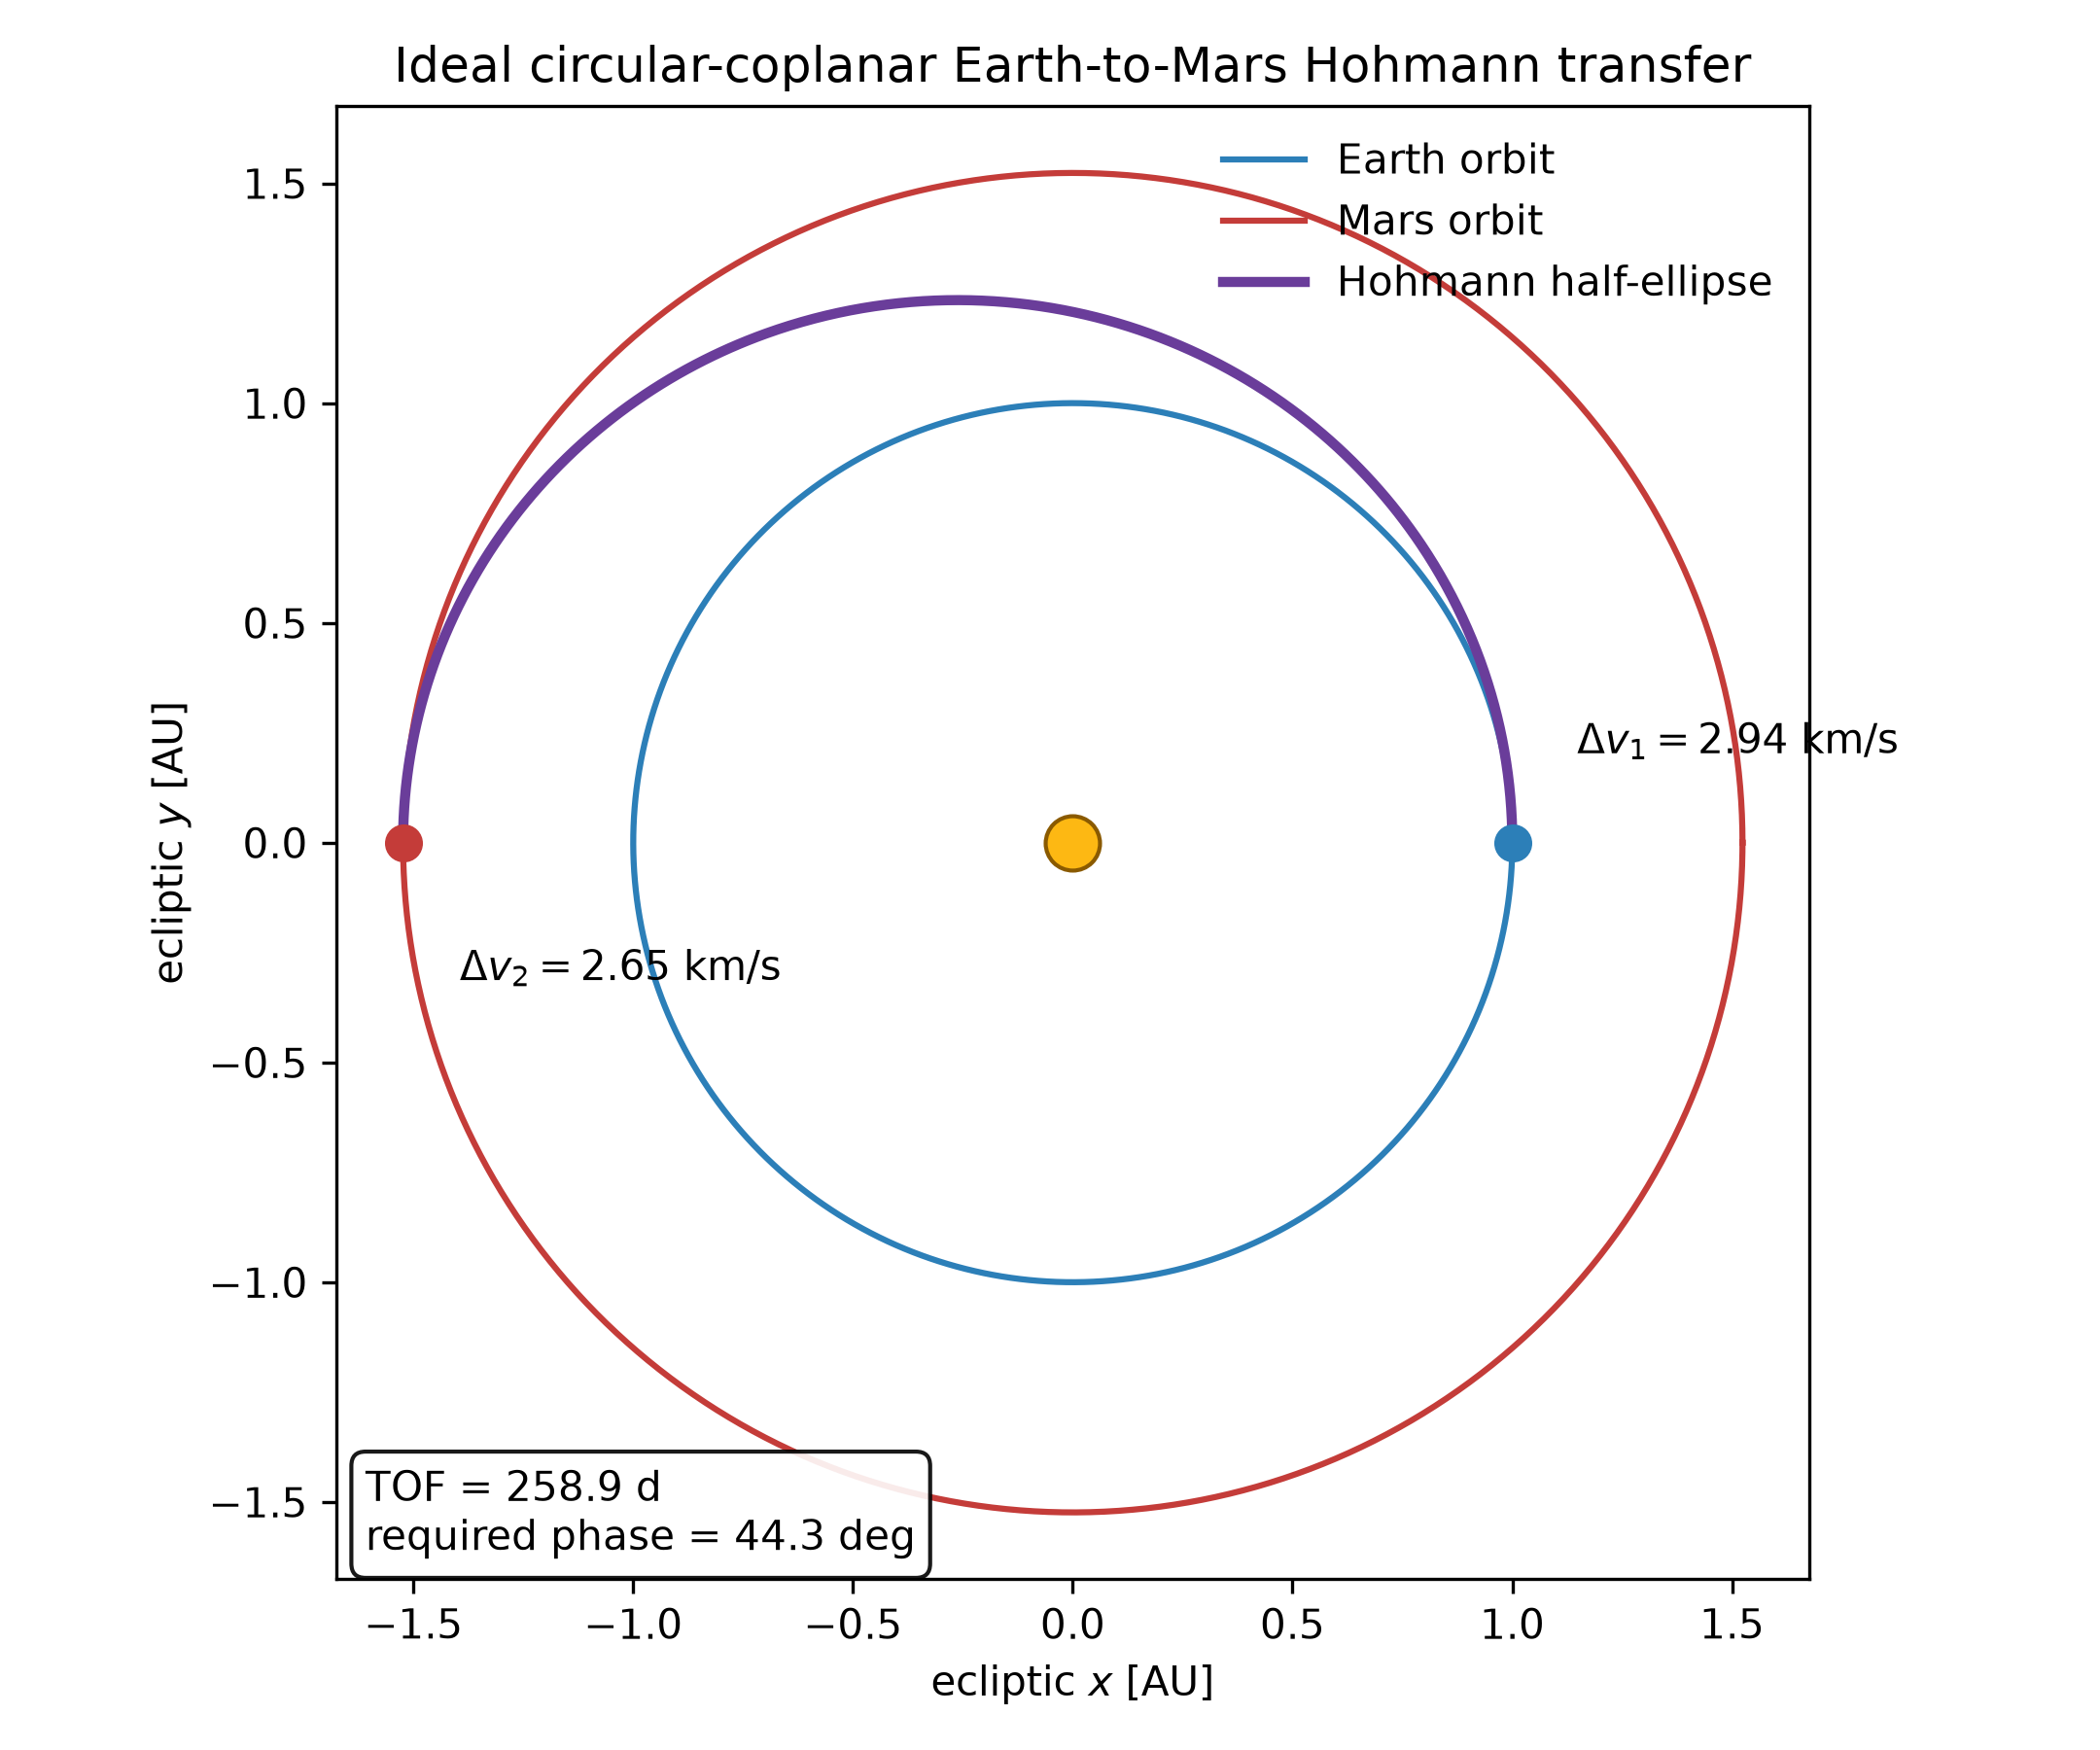
\includegraphics[width=0.85\textwidth]{hohmann_transfer.png}
    \caption{Ideal Circular-Coplanar Earth-Mars Hohmann Transfer Geometry, showing Earth circular orbit, Mars circular orbit and the tangent transfer ellipse with two impulse manoeuvres.}
    \label{fig:hohmann_geo}
\end{figure}

\section{Ephemeris-Driven Lambert Transfer Model}
\label{sec:lambert-model}

\subsection{From the Analytic Benchmark to Date-Specific Design}

The preceding Hohmann analysis provides a transparent benchmark for the
characteristic velocity scale and flight time of an idealized Earth--Mars
transfer. Its circular, coplanar geometry does not, however, determine the
planetary position and velocity vectors on a specified calendar date. A launch
window is therefore not obtained by drawing a single tangent half-ellipse, but
by solving a two-point orbital boundary-value problem over many possible
combinations of departure date and arrival date.

We develop the date-specific model in three levels. The first is a
phase-anchored circular--coplanar model, retained to show the connection with
the Hohmann benchmark. The second uses the secular Keplerian elements published
by JPL from the Standish--Williams approximation. The third and principal model
uses Cartesian states from the integrated DE440s ephemeris. This hierarchy
separates two questions: whether a simple approximation identifies the same
broad low-energy opportunity, and whether its boundary states are sufficiently
accurate to select a refined mission date.

\subsection{Secular Keplerian Approximation}
\label{sec:standish-model}

A natural intermediate model is to approximate each planetary orbit by six
Keplerian elements and their secular rates. For a Julian ephemeris date
$T_{\mathrm{eph}}$, measured on the TDB timescale, define the number of Julian
centuries after J2000.0 by
\begin{equation}
  T=\frac{T_{\mathrm{eph}}-2451545.0}{36525}.
\end{equation}
For each element
\begin{equation}
  q\in\{a,e,I,L,\varpi,\Omega\},
\end{equation}
the 1800--2050 approximation has the form
\begin{equation}
  q(T)=q_0+\dot q\,T,
  \label{eq:standish-elements}
\end{equation}
where $a$ is the semi-major axis, $e$ is the eccentricity, $I$ is the
inclination, $L$ is the mean longitude, $\varpi$ is the longitude of
perihelion, and $\Omega$ is the longitude of the ascending node
\cite{standish1992,jplapprox}. For Earth and Mars in this time interval, the
mean anomaly and argument of perihelion are
\begin{equation}
  M=L-\varpi,
  \qquad
  \omega=\varpi-\Omega.
\end{equation}
The eccentric anomaly $E$ is obtained from Kepler's equation
\begin{equation}
  M=E-e\sin E,
  \label{eq:standish-kepler}
\end{equation}
and the coordinates in the orbital plane are
\begin{equation}
  x'=a(\cos E-e),
  \qquad
  y'=a\sqrt{1-e^2}\sin E,
  \qquad
  z'=0.
\end{equation}
Writing $c_x=\cos x$ and $s_x=\sin x$, the corresponding J2000 ecliptic
coordinates are evaluated with the explicit transformation
\begin{equation}
\begin{bmatrix}
 x\\y\\z
\end{bmatrix}
=
\begin{bmatrix}
 c_\omega c_\Omega-s_\omega s_\Omega c_I &
 -s_\omega c_\Omega-c_\omega s_\Omega c_I\\
 c_\omega s_\Omega+s_\omega c_\Omega c_I &
 -s_\omega s_\Omega+c_\omega c_\Omega c_I\\
 s_\omega s_I & c_\omega s_I
\end{bmatrix}
\begin{bmatrix}
 x'\\y'
\end{bmatrix}.
\label{eq:standish-rotation}
\end{equation}
The approximate velocities are obtained by a centred difference of the
position model with a step of $0.05$ day. Halving this step changes the
reported transfer metrics below their displayed precision.

The JPL table represents the Earth--Moon barycentre rather than the terrestrial
geocentre. It is also a fitted low-accuracy representation rather than an
integrated ephemeris. JPL lists nominal distance errors of approximately
$6000\,\mathrm{km}$ for the Earth--Moon barycentre and
$25000\,\mathrm{km}$ for Mars over 1800--2050 and explicitly recommends a
high-precision ephemeris when greater accuracy is required
\cite{jplapprox}. We therefore use this model as a screening and corroboration
tool, not as the final source of mission boundary states.

\begin{figure}[H]
  \centering
  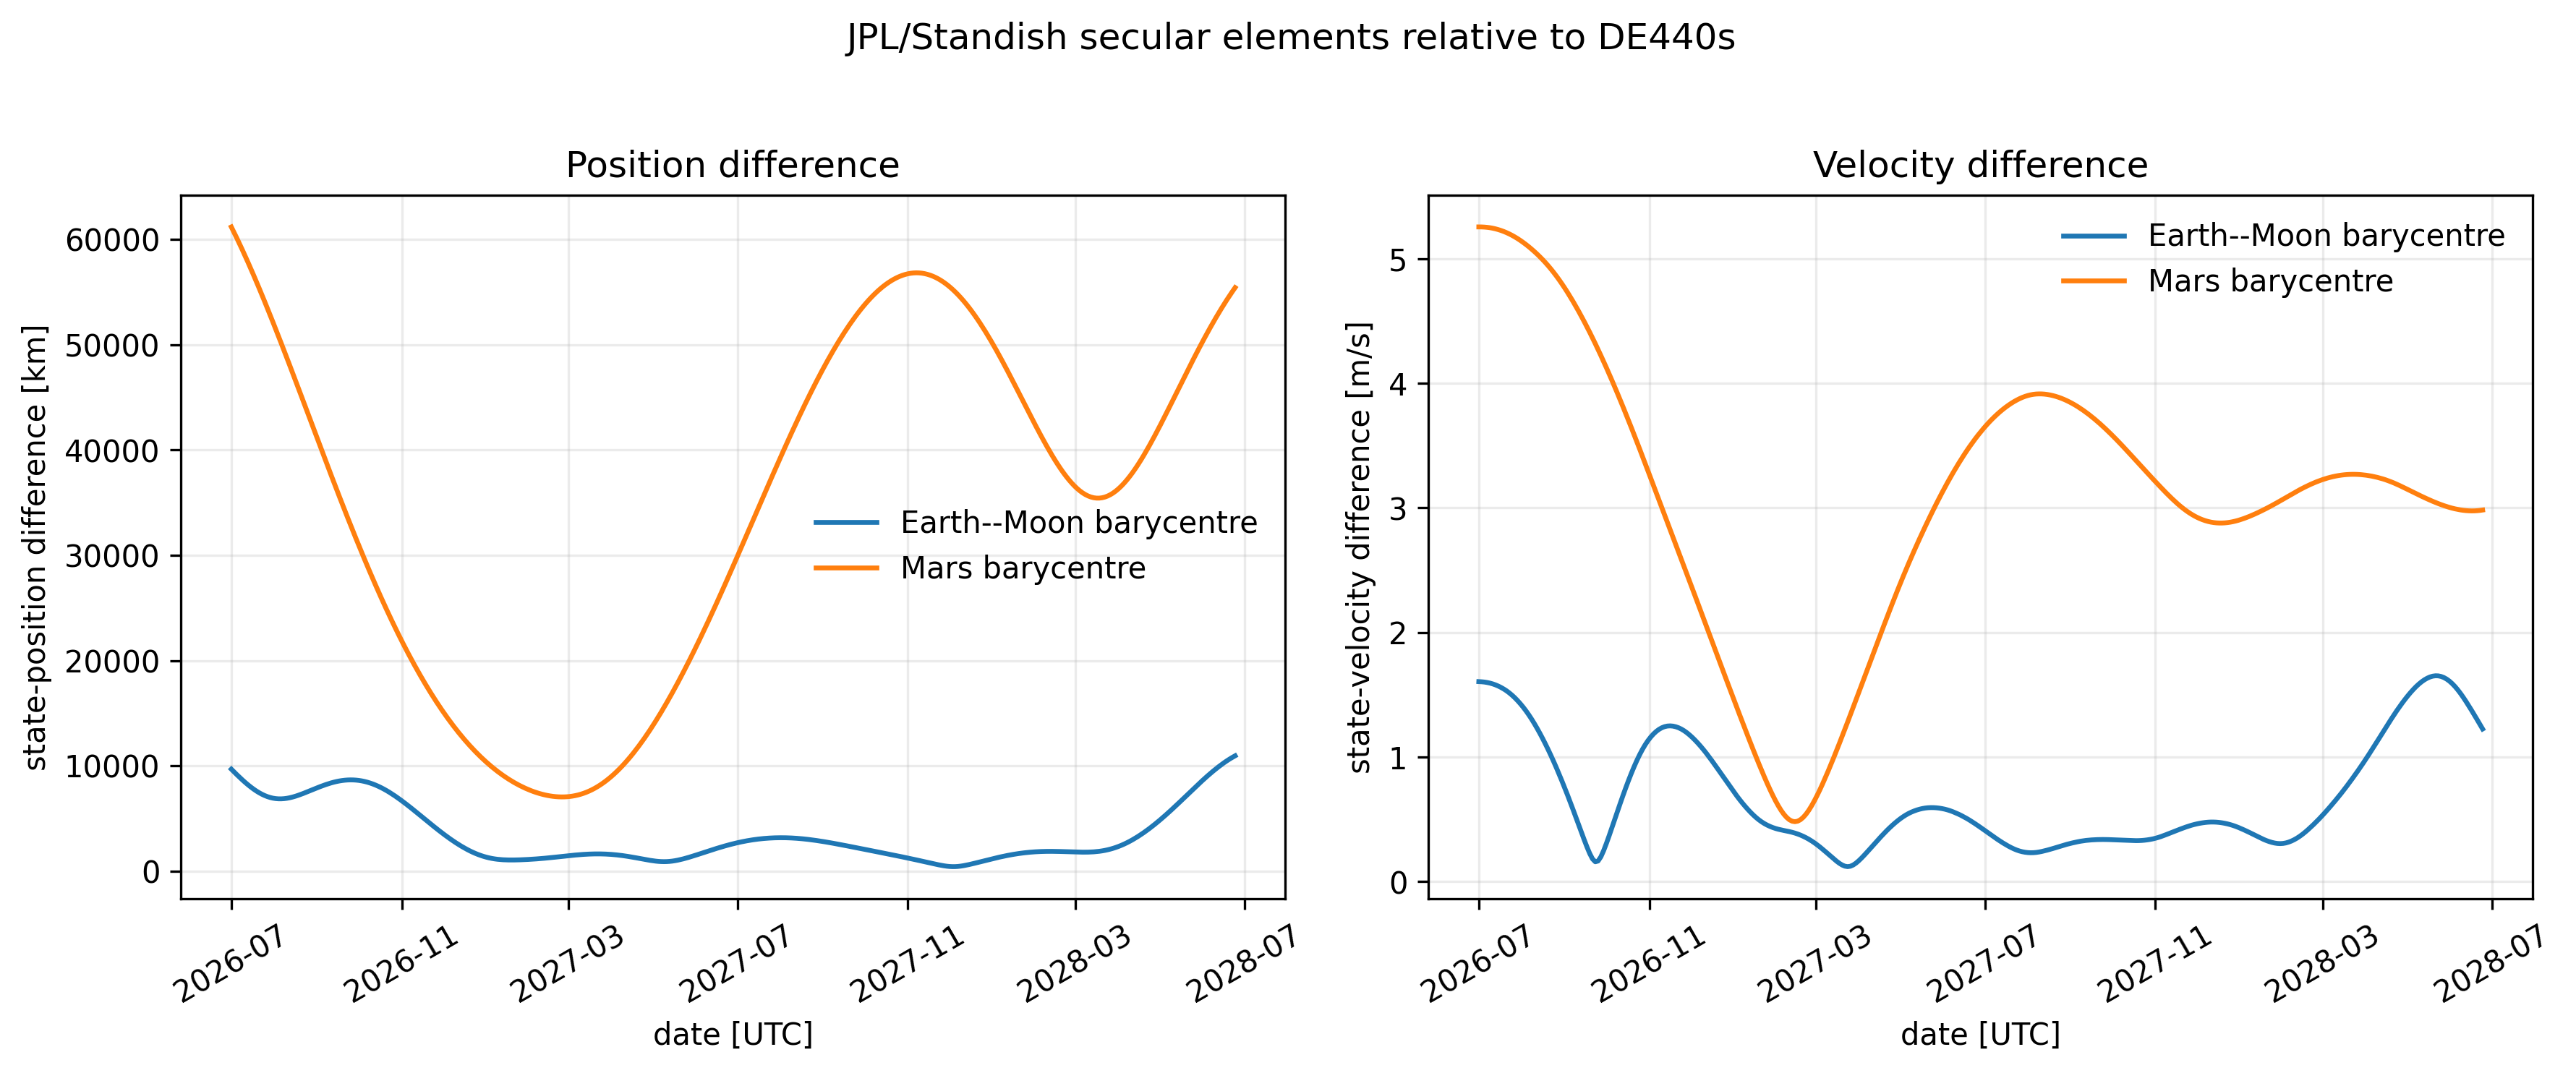
\includegraphics[width=\textwidth]{standish_de440s_state_difference.png}
  \caption{Differences between the JPL/Standish secular-element states and DE440s over the complete time interval sampled by the transfer search. The Earth curve compares the approximate Earth--Moon barycentre with the DE440s Earth barycentre; the Mars curve compares the corresponding Mars barycentre states. Left: Euclidean position difference. Right: Euclidean velocity difference. Source: authors' calculations.}
  \label{fig:standish-state-difference}
\end{figure}

Figure~\ref{fig:standish-state-difference} shows that the Earth--Moon
barycentre position difference has a median of
$\StandishEarthMedianPositionError\,\mathrm{km}$ and a maximum of
$\StandishEarthMaximumPositionError\,\mathrm{km}$, while the corresponding
Mars values are $\StandishMarsMedianPositionError\,\mathrm{km}$ and
$\StandishMarsMaximumPositionError\,\mathrm{km}$. The median velocity
differences are $\StandishEarthMedianVelocityError\,\mathrm{m\,s^{-1}}$ and
$\StandishMarsMedianVelocityError\,\mathrm{m\,s^{-1}}$, respectively. These
errors are small relative to heliocentric distances and orbital speeds, but are
not negligible when neighbouring launch dates are compared.

\subsection{DE440s Boundary States and Reference Conventions}
\label{sec:de440s-states}

The principal model obtains planetary states from NASA/JPL DE440s through the
NAIF SPICE toolkit \cite{park2021,acton1996,naifkernels}. User-facing calendar
dates are specified in UTC and converted by SPICE to ephemeris time, whose
underlying independent variable is TDB. Geometric states are requested in the
\code{ECLIPJ2000} frame with the Sun as observer and with aberration correction
set to \code{NONE}. The departure state is the terrestrial geocentre
\code{EARTH}. The compact DE440s kernel supplies the Martian system state as
\code{MARS BARYCENTER}, which is used for the arrival boundary. Positions and
velocities are expressed in kilometres and kilometres per second.

The distinction between the models is important. The Standish approximation
uses a small set of time-varying orbital elements and therefore captures the
main eccentricity, inclination, and phasing effects. DE440s instead stores
Chebyshev representations of numerically integrated Cartesian states and is
designed to support high-precision planetary calculations \cite{park2021}.
The approximate model can therefore corroborate the location and scale of a
solution, whereas DE440s is better suited to the final date-specific search.

\subsection{Lambert Boundary-Value Formulation}
\label{sec:lambert-formulation}

For a departure epoch $t_1$ and an arrival epoch $t_2$, the planetary state
model supplies
\begin{equation}
  \vect r_1=\vect r_E(t_1),
  \qquad
  \vect r_2=\vect r_M(t_2),
  \qquad
  \Delta t=t_2-t_1.
\end{equation}
Lambert's problem determines the heliocentric spacecraft velocities
$\vect v_1$ and $\vect v_2$ that connect the two prescribed position vectors in
the prescribed time. Our implementation uses the zero-revolution prograde
universal-variable formulation described by Vallado and Curtis
\cite{vallado2013,curtis2020}. Transfer angles greater than $\pi$ are retained
when required by the endpoint geometry, so the selected prograde branch may be
a long-way transfer.

Let $\Delta\theta$ denote the selected transfer angle and define
\begin{equation}
  A=\sin\Delta\theta
  \sqrt{\frac{r_1r_2}{1-\cos\Delta\theta}}.
\end{equation}
The Stumpff functions are evaluated as
\begin{equation}
C(z)=
\begin{cases}
\dfrac{1-\cos\sqrt z}{z}, & z>0,\\[5pt]
\dfrac12, & z=0,\\[5pt]
\dfrac{\cosh\sqrt{-z}-1}{-z}, & z<0,
\end{cases}
\end{equation}
\begin{equation}
S(z)=
\begin{cases}
\dfrac{\sqrt z-\sin\sqrt z}{(\sqrt z)^3}, & z>0,\\[5pt]
\dfrac16, & z=0,\\[5pt]
\dfrac{\sinh\sqrt{-z}-\sqrt{-z}}{(\sqrt{-z})^3}, & z<0.
\end{cases}
\end{equation}
Near $z=0$, truncated power series are used to avoid subtractive cancellation.
The auxiliary functions are
\begin{align}
  y(z) &= r_1+r_2+A\frac{zS(z)-1}{\sqrt{C(z)}},\\
  F(z) &= \left(\frac{y(z)}{C(z)}\right)^{3/2}S(z)
       +A\sqrt{y(z)}-\sqrt{\mu_\odot}\,\Delta t.
\end{align}
A finite interval with a sign change is first constructed. The root of
$F(z)=0$ is then found with Brent's bracketing method using absolute and
relative tolerances of $10^{-11}$ and $10^{-13}$, respectively. Candidates
with invalid $C(z)$, non-positive $y(z)$, singular geometry, or a vanishing
Lagrange coefficient are rejected. Once the root is known,
\begin{equation}
  f=1-\frac{y}{r_1},
  \qquad
  g=A\sqrt{\frac{y}{\mu_\odot}},
  \qquad
  \dot g=1-\frac{y}{r_2},
\end{equation}
so that
\begin{equation}
  \vect v_1=\frac{\vect r_2-f\vect r_1}{g},
  \qquad
  \vect v_2=\frac{\dot g\vect r_2-\vect r_1}{g}.
\end{equation}

\begin{figure}[H]
  \centering
  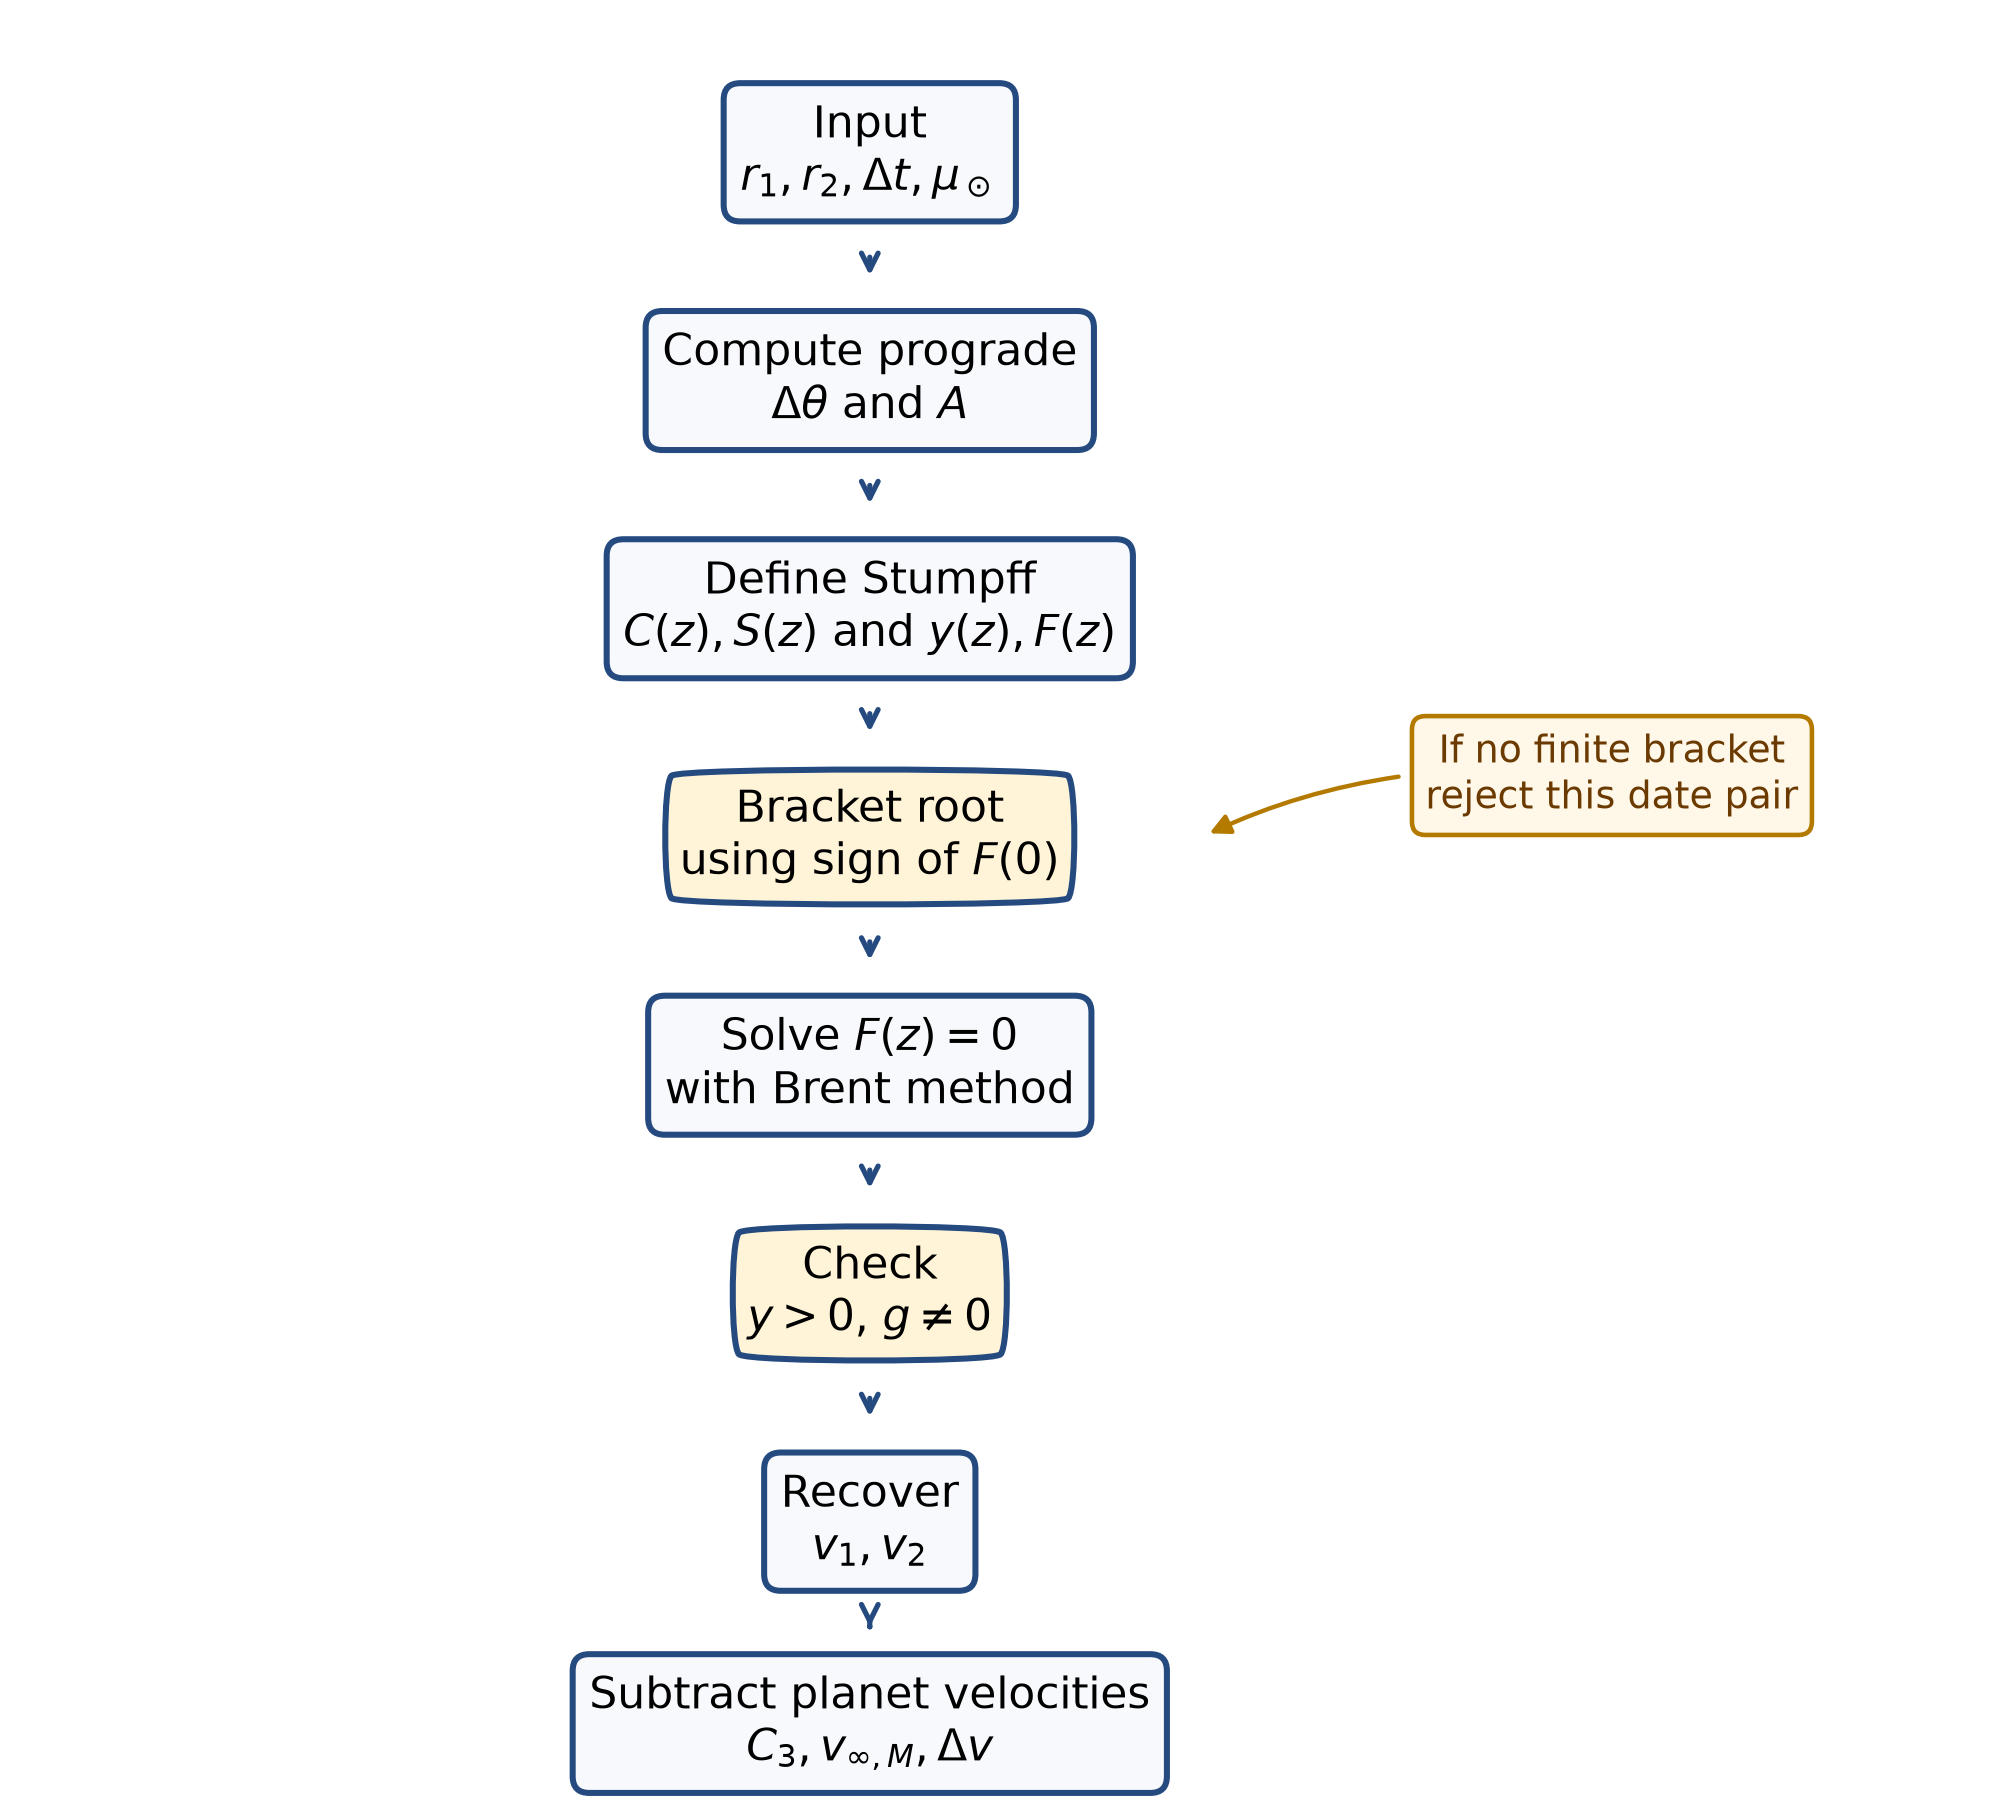
\includegraphics[width=0.88\textwidth]{lambert_solver_flowchart.png}
  \caption{Numerical sequence used for each Lambert boundary-value solve. The algorithm selects the prograde transfer angle, constructs and brackets the universal-variable residual, applies Brent's method, checks the Lagrange coefficients, and recovers the endpoint velocities. Source: authors' implementation.}
  \label{fig:flowchart}
\end{figure}

\subsection{Mission Metrics and Search Procedure}
\label{sec:mission-metrics}

The endpoint excess-velocity vectors are
\begin{equation}
  \vect v_{\infty,E}=\vect v_1-\vect v_E(t_1),
  \qquad
  \vect v_{\infty,M}=\vect v_2-\vect v_M(t_2),
\end{equation}
and the Earth-departure characteristic energy is
\begin{equation}
  C_3=\norm{\vect v_{\infty,E}}^2.
\end{equation}
To compare complete transfer opportunities with one consistent scalar metric,
we use impulsive patched-conic injection from a $200\,\mathrm{km}$ circular
low Earth orbit and impulsive capture into a $250\,\mathrm{km}$ circular low
Mars orbit. For a parking-orbit radius $r_p$, the required impulse is
\begin{equation}
  \Delta v_p=
  \sqrt{v_\infty^2+\frac{2\mu}{r_p}}
  -\sqrt{\frac{\mu}{r_p}},
\end{equation}
and the adopted two-impulse budget is
\begin{equation}
  \Delta v_{\mathrm{total}}
  =\Delta v_{\mathrm{LEO}}+\Delta v_{\mathrm{LMO}}.
  \label{eq:patched-total}
\end{equation}
This is a comparison metric rather than a complete vehicle budget: it excludes
launch-site geometry, finite burns, midcourse corrections, atmospheric entry,
aerocapture, landing, and spacecraft mass staging.

The production search samples departures from 2026-07-01 through 2027-06-30
at two-day intervals and times of flight from 140 to 360 days at two-day
intervals. The minima of $C_3$ and total $\Delta v$ are then refined in a
$\pm6$ day neighbourhood with a $0.25$ day mesh in departure epoch and time of
flight. A grid point is retained whenever the Lambert solve and the derived
metrics are finite; no arbitrary hyperbolic-excess-speed threshold is imposed.

\subsection{Numerical Verification}
\label{sec:q3-verification}

The solver is checked in four complementary ways. First, a regression test
reproduces the standard Vallado universal-variable Lambert example. Second,
the recommended departure state is propagated independently with a high-order
DOP853 integrator; the propagated endpoint differs from the prescribed Mars
position by only $\LambertEndpointError\,\mathrm{km}$. Third, the grid is
coarsened and then locally refined to verify convergence of the reported
minimum.

\begin{table}[H]
\centering
\caption{Grid-resolution check for the minimum-total-$\Delta v$ solution. Source: authors' calculations.}
\label{tab:grid-convergence}
\scriptsize
\begin{tabular}{lrrr}
\toprule
Resolution & Departure [UTC] & TOF [d] & Total $\Delta v$ [km/s] \\
\midrule
4-day subsample & 2026-11-02 & 308.00 & 5.696353 \\
2-day production grid & 2026-11-02 & 310.00 & 5.695948 \\
local 0.25-day refinement & 2026-11-01 & 310.25 & 5.695651 \\
\bottomrule
\end{tabular}
\end{table}

Finally, the Standish boundary-state model provides a structurally different
approximation to the same launch opportunity. Agreement between its optimum and
the DE440s optimum does not prove the Lambert implementation by itself, since
the same solver is used, but it gives an independent physical check that the
low-energy valley is not an artifact of one ephemeris representation.

\section{Launch-Window Results and Mission Trade-offs}
\label{sec:launch-window}

\subsection{Porkchop Maps for the 2026--2027 Opportunity}

A porkchop map places departure date on the horizontal axis and arrival date on
the vertical axis; every valid point represents one Lambert solution.
Figure~\ref{fig:porkchop-main} displays the DE440s results. The left panel
shows launch $C_3$, while the right panel shows the two-impulse patched-conic
budget. Dashed diagonal lines indicate constant time of flight. Values above
the displayed colour range are clipped only to preserve contrast in the
low-cost valley and are not treated as infeasible.

\begin{figure}[H]
  \centering
  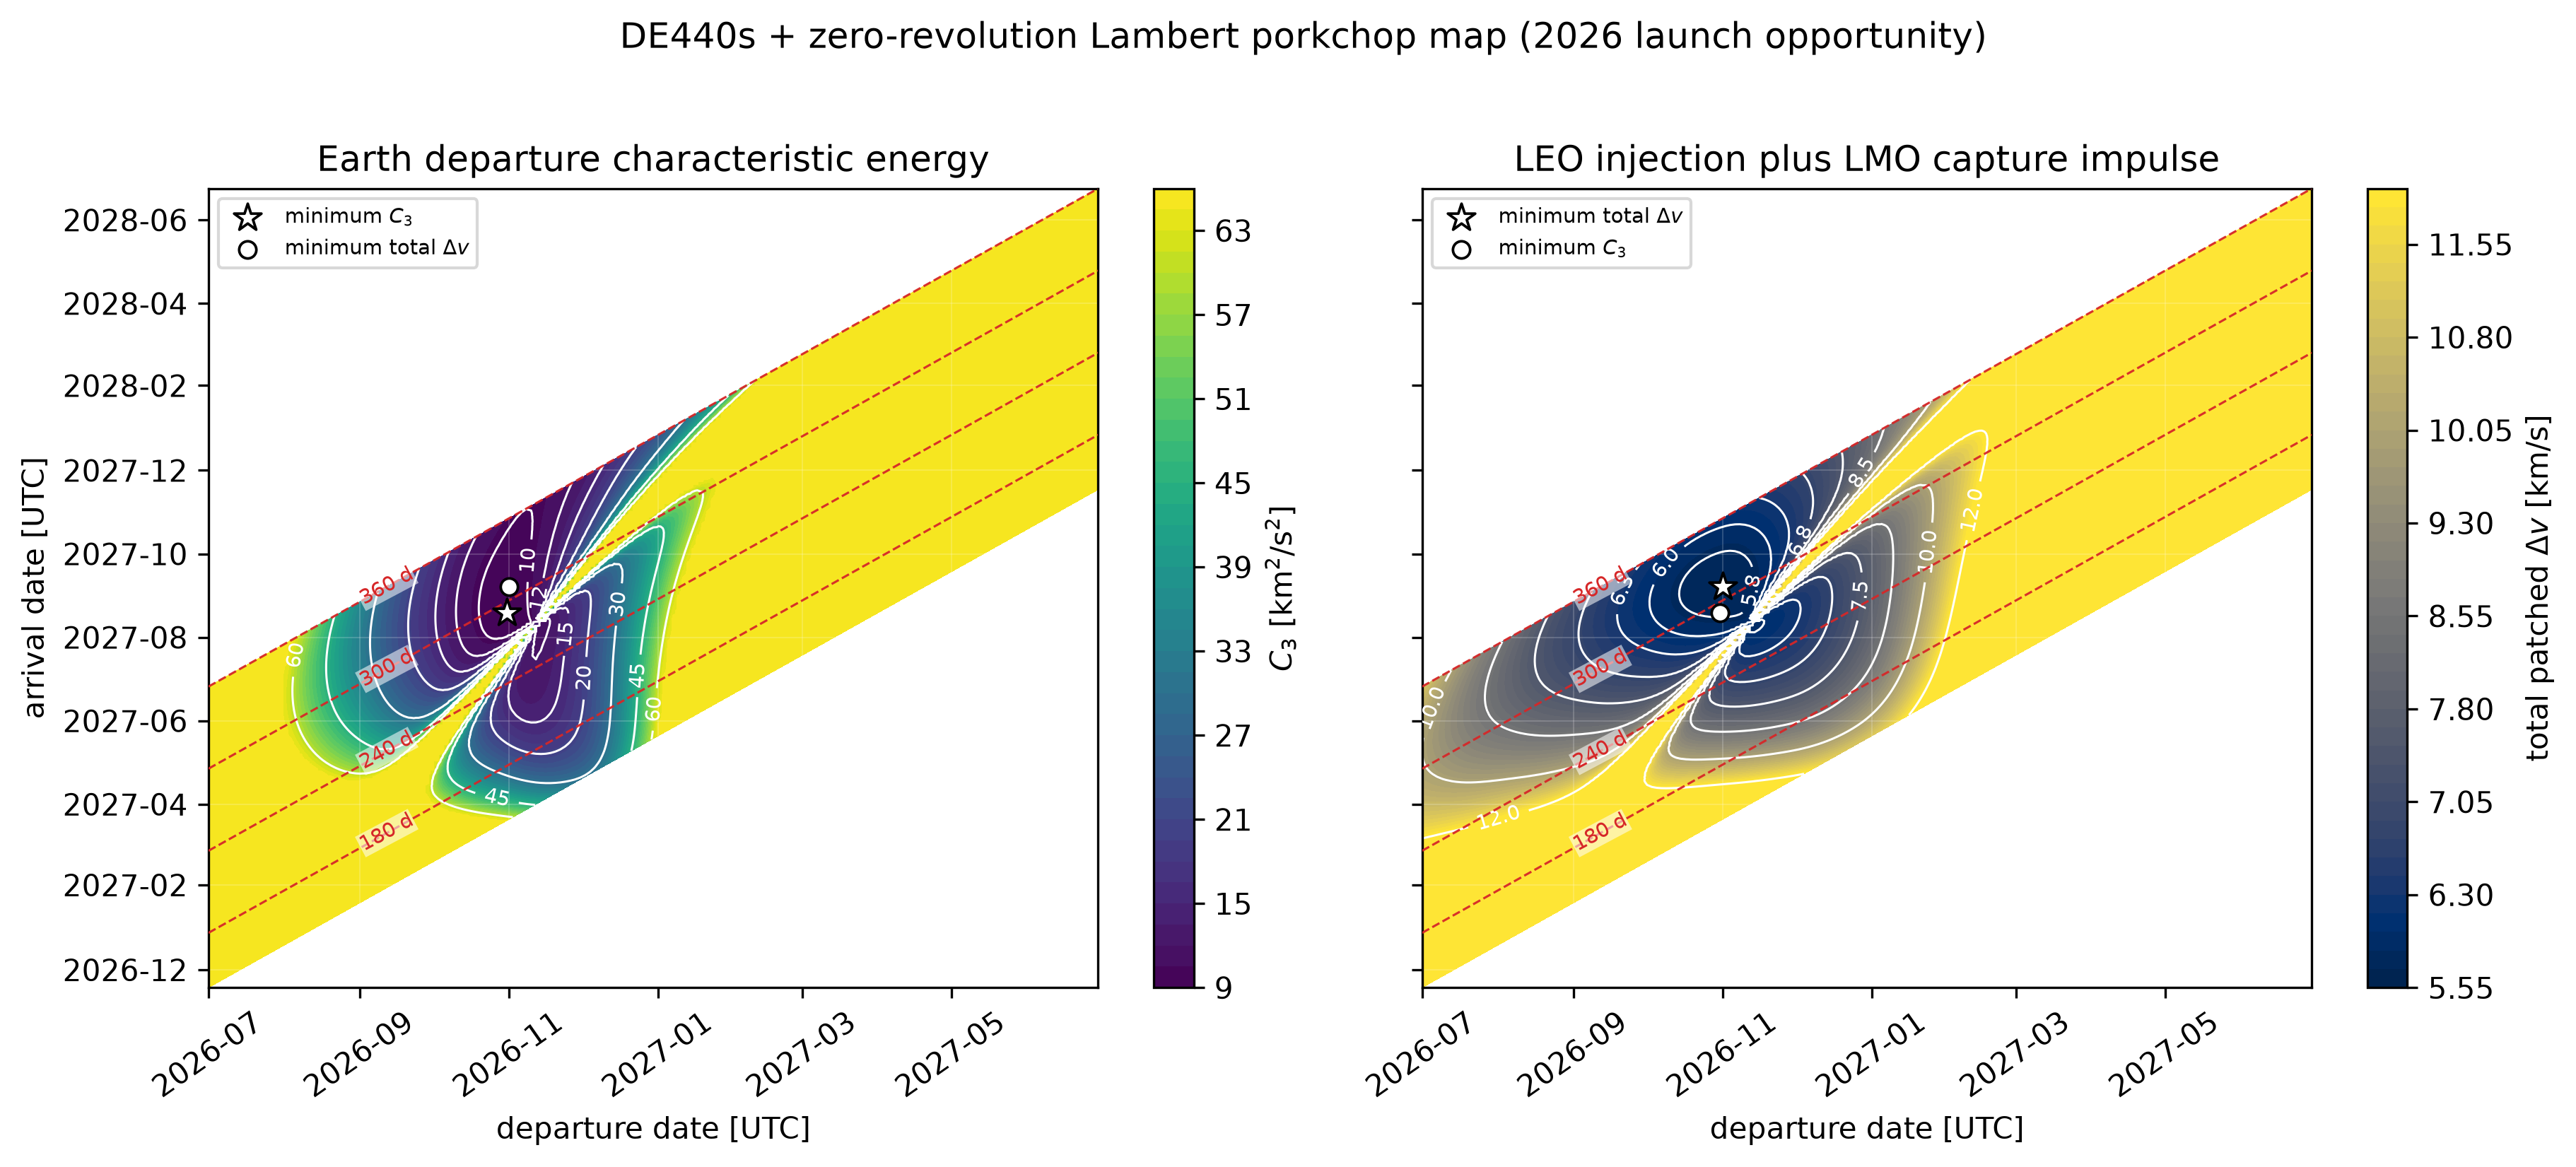
\includegraphics[width=\textwidth]{porkchop_2026_2027.png}
  \caption{DE440s zero-revolution prograde Lambert porkchop maps. Left: Earth-departure characteristic energy $C_3$. Right: injection from a $200\,\mathrm{km}$ circular LEO plus capture into a $250\,\mathrm{km}$ circular LMO. In each panel, the star marks the minimum of the displayed metric and the circle marks the minimum of the other metric. Red dashed lines show constant time of flight. Source: authors' calculations.}
  \label{fig:porkchop-main}
\end{figure}

The phase-anchored circular--coplanar calculation in
Figure~\ref{fig:model-comparison} preserves the broad Hohmann-like valley but
moves its centre because it suppresses eccentricity, inclination, and radial
variation. It is therefore useful as a baseline, not as a calendar-level launch
prediction.

\begin{figure}[H]
  \centering
  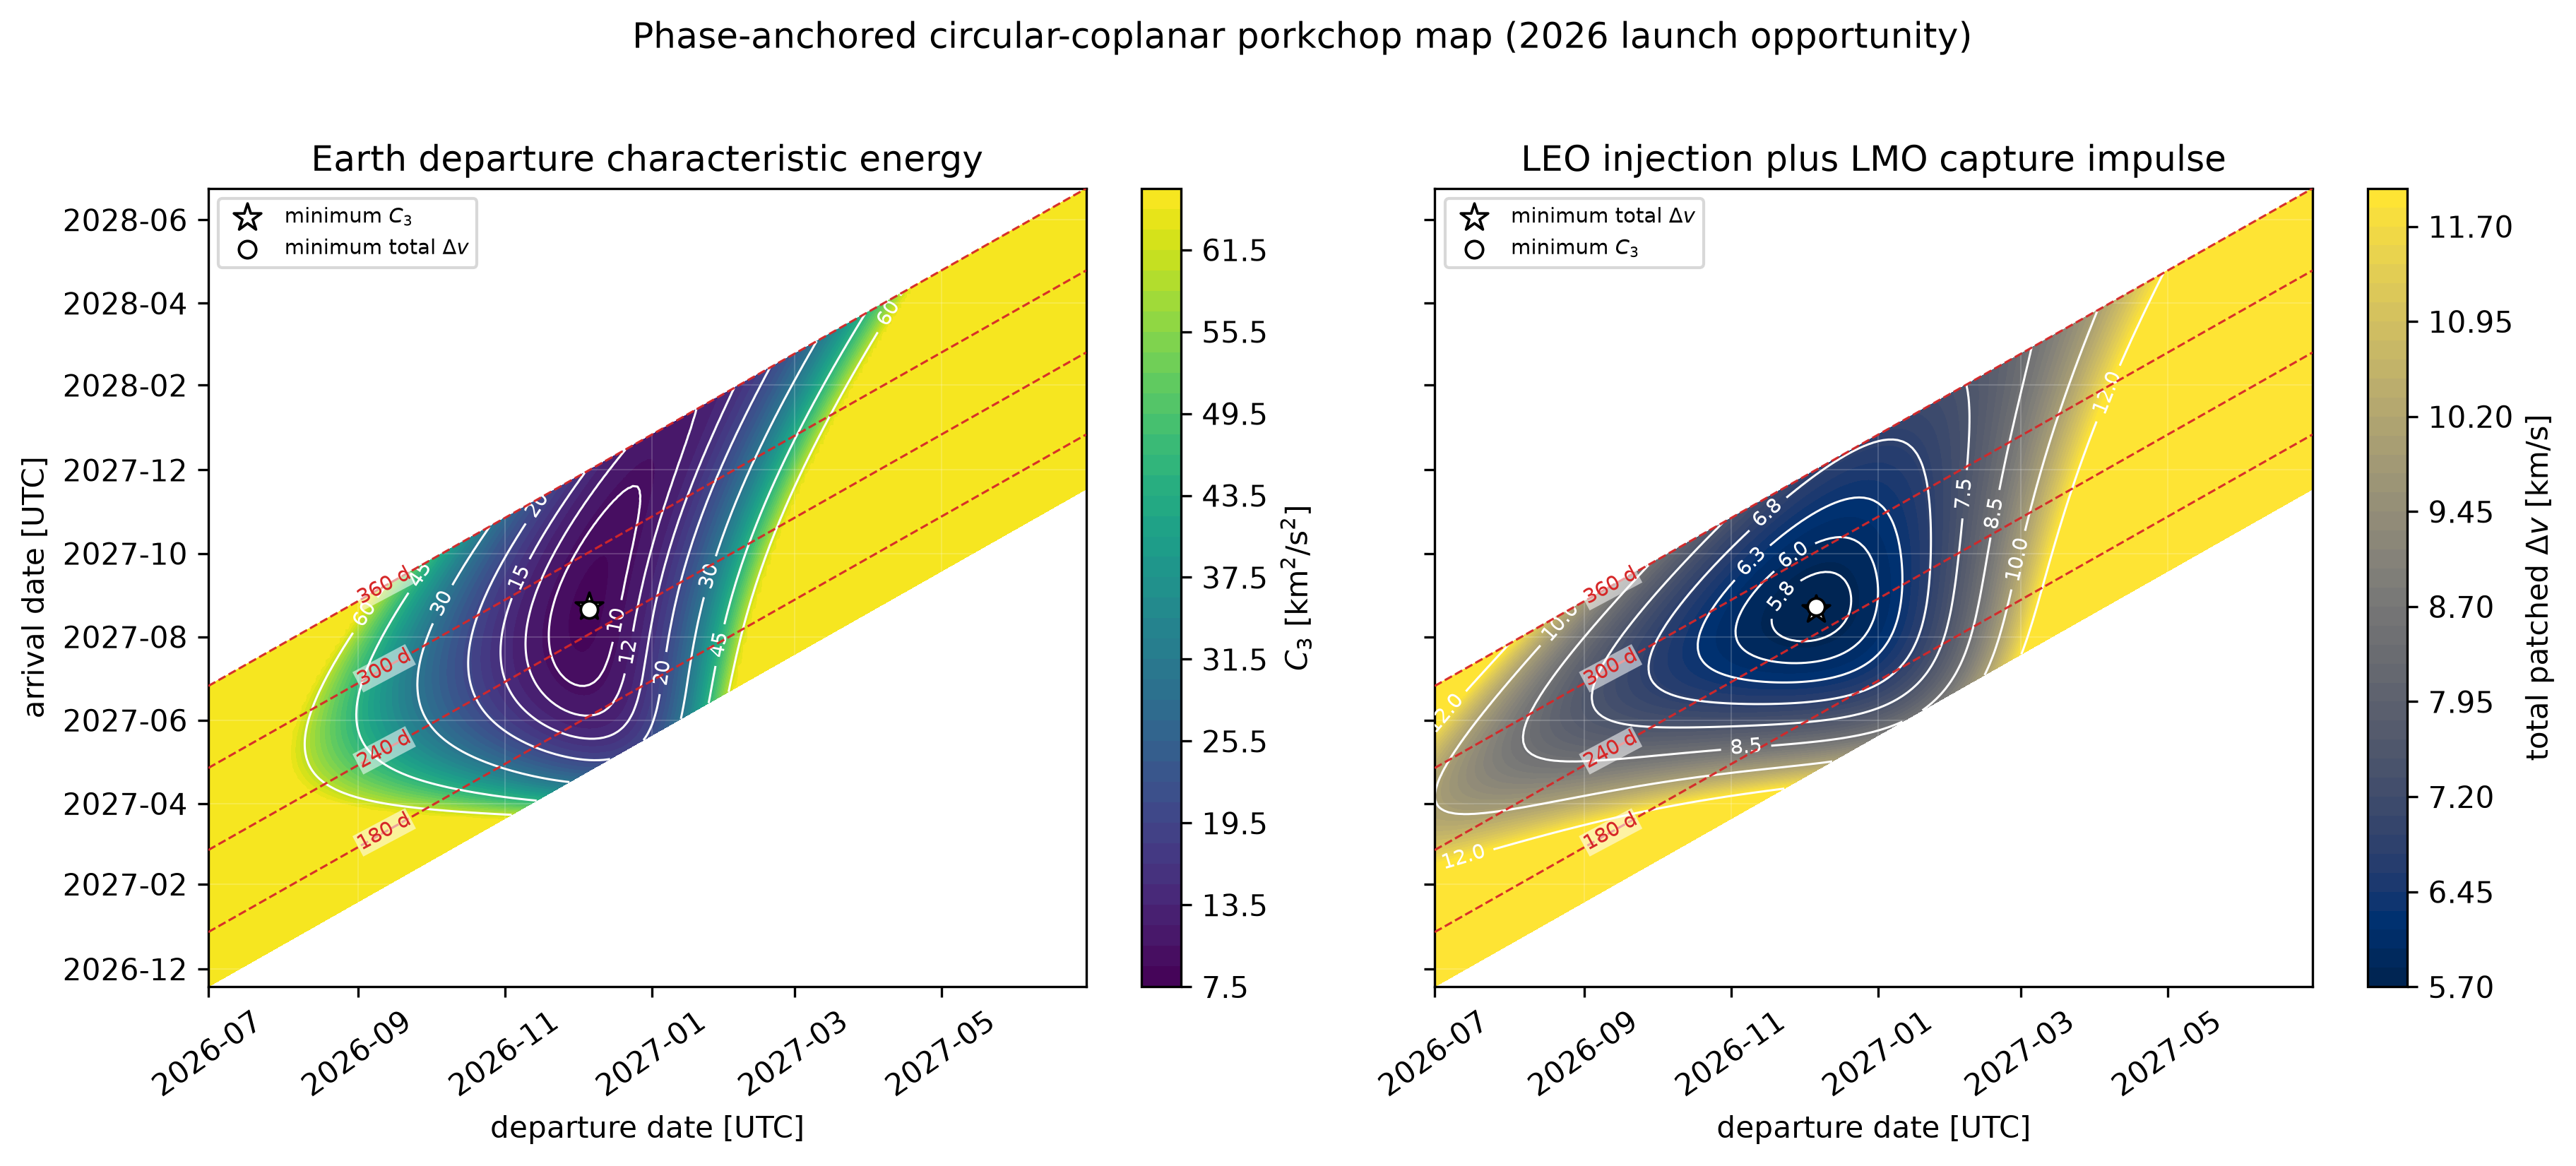
\includegraphics[width=\textwidth]{porkchop_circular_coplanar_2026_2027.png}
  \caption{Phase-anchored circular--coplanar porkchop maps over the same date and time-of-flight domain as Figure~\ref{fig:porkchop-main}. The planetary longitudes are anchored to DE440s at the beginning of the search, after which both planets move on fixed circular orbits. Source: authors' calculations.}
  \label{fig:model-comparison}
\end{figure}

\subsection{Comparison of the Three State Models}

\begin{table}[H]
\centering
\caption{Minimum-total-$\Delta v$ solutions obtained with the circular--coplanar, JPL/Standish, and DE440s state models. The circular result is selected on the two-day production grid; the Standish and DE440s minima include the $0.25$ day local refinement. Source: authors' calculations.}
\label{tab:model-levels}
\scriptsize
\begin{tabular}{lccrrr}
\toprule
Planetary-state model & Departure & Arrival & TOF [d] & $C_3$ & Total $\Delta v$ [km/s] \\
\midrule
Circular--coplanar & 2026-12-06 & 2027-08-21 & 258.00 & 8.68 & 5.708 \\
JPL/Standish secular elements & 2026-10-31 06:00 & 2027-09-07 06:00 & 311.00 & 9.23 & 5.695 \\
DE440s ephemeris & 2026-11-01 06:00 & 2027-09-07 12:00 & 310.25 & 9.27 & 5.696 \\
\bottomrule
\end{tabular}
\end{table}

The circular--coplanar result flies for $\CircularMinimumTOF$ days, close to
the Hohmann value of $\HohmannTOF$ days. Its total impulse is nevertheless
close to the DE440s minimum, showing that the ideal model captures the
characteristic energy scale even though it does not locate the same dates.

The Standish minimum departs at \StandishMinimumDeparture{} UTC and differs
from the DE440s optimum by only \RealMinusStandishDepartureDays{} day in
departure epoch, $\lvert\RealMinusStandishTOF\rvert$ day in flight time, and
$\lvert\RealMinusStandishDV\rvert\,\mathrm{km\,s^{-1}}$ in the adopted
impulse metric. This agreement further supports the location and cost scale of
the DE440s low-energy valley. At the same time, the state differences in
Figure~\ref{fig:standish-state-difference}, the use of the Earth--Moon
barycentre, and the day-scale shift of the refined optimum justify retaining
DE440s for the final mission dates.

\subsection{Candidate Selection under Competing Objectives}

No single transfer simultaneously minimizes launch energy, total parking-orbit
impulse, and flight time. To remain consistent with the companion project
website and its reported design set, the comparison below uses the same
low-to-moderate-energy analysis domain,
\begin{equation}
  v_{\infty,E}<12\,\mathrm{km\,s^{-1}},
  \qquad
  v_{\infty,M}<12\,\mathrm{km\,s^{-1}}.
  \label{eq:candidate-domain}
\end{equation}
This bound is a declared screening convention rather than a universal physical
feasibility limit. Its purpose is to exclude extreme high-energy solutions from
the mission-comparison plot while preserving the launch opportunity relevant to
the four designs used throughout the report and the website.

Within this common domain, four complementary selection rules are retained:
\begin{itemize}
  \item \textbf{Minimum total $\Delta v$:} minimizes the two-impulse
  parking-orbit budget in Eq.~\eqref{eq:patched-total}. This is the principal
  recommendation when propellant is the dominant objective.
  \item \textbf{Minimum launch $C_3$:} minimizes the characteristic energy at
  Earth departure without requiring the Mars-capture impulse to be minimal.
  \item \textbf{Fast (within 0.5 km/s):} first restricts the common candidate
  set to transfers satisfying
  $\Delta v_{\mathrm{total}}\leq\Delta v_{\min}+0.5\,\mathrm{km\,s^{-1}}$,
  and then selects the shortest flight. This is a schedule-priority scenario,
  not a universal optimum.
  \item \textbf{Balanced Pareto design:} constructs the strict nondominated
  frontier in time of flight and total $\Delta v$, normalizes both coordinates
  to $[0,1]$, and selects the point closest to the equal-weight utopia point.
\end{itemize}

\begin{table}[H]
\centering
\caption{Representative DE440s designs for the 2026 launch opportunity. The four selection types and their reported values are kept consistent with the companion project website. $C_3$ is in $\mathrm{km^2\,s^{-2}}$, while $v_{\infty,M}$ and total $\Delta v$ are in $\mathrm{km\,s^{-1}}$. Source: authors' calculations.}
\label{tab:candidates}
\scriptsize
\begin{tabular}{p{0.20\textwidth}llrrrr}
\toprule
Design & Departure & Arrival & TOF [d] & $C_3$ & $v_{\infty,M}$ & Total $\Delta v$ \\
\midrule
Minimum total $\Delta v$ & 2026-11-01 06:00 & 2027-09-07 12:00 & 310.2 & 9.27 & 2.57 & 5.696 \\
Minimum launch $C_3$ & 2026-10-31 12:00 & 2027-08-19 18:00 & 292.2 & 9.18 & 2.72 & 5.763 \\
Fast (within 0.5 km/s) & 2026-11-18 & 2027-07-28 & 252.0 & 12.68 & 3.21 & 6.172 \\
Balanced Pareto design & 2026-12-06 & 2027-06-26 & 202.0 & 23.04 & 4.52 & 7.427 \\
\bottomrule
\end{tabular}
\end{table}

The minimum-total-$\Delta v$ design departs at \MinimumDeparture{} UTC,
arrives at \MinimumArrival{} UTC, and flies for \MinimumTOF{} days. It requires
\MinimumLEODV\kms{} for LEO injection and \MinimumLMODV\kms{} for LMO capture,
giving \MinimumTotalDV\kms{} in total. The signed relative difference in this impulse metric, computed as DE440s
minus the circular Hohmann benchmark, is \ActualDVPenaltyPercent\%, while the
flight time is \ActualTOFPenaltyPercent\% longer. The
important discrepancy is therefore not the first-order impulse scale, but the
calendar geometry and time of flight.

The $0.5\,\mathrm{km\,s^{-1}}$ allowance in the fast design is a modelling
choice. Table~\ref{tab:fast-threshold} shows how the selected schedule changes
when this allowance is varied while the common analysis domain in
Eq.~\eqref{eq:candidate-domain} is retained.

\begin{table}[H]
\centering
\caption{Sensitivity of the Fast (within 0.5 km/s) selection rule to the allowed total-$\Delta v$ increase above the production-grid minimum. The $0.5\,\mathrm{km\,s^{-1}}$ row is the design retained in Table~\ref{tab:candidates}. Source: authors' calculations.}
\label{tab:fast-threshold}
\scriptsize
\begin{tabular}{rccrr}
\toprule
Allowed excess [km/s] & Departure & Arrival & TOF [d] & Total $\Delta v$ [km/s] \\
\midrule
0.25 & 2026-11-14 & 2027-08-11 & 270 & 5.936 \\
0.50 & 2026-11-18 & 2027-07-28 & 252 & 6.172 \\
0.75 & 2026-11-24 & 2027-07-20 & 238 & 6.433 \\
1.00 & 2026-11-28 & 2027-07-14 & 228 & 6.657 \\
\bottomrule
\end{tabular}
\end{table}

The table makes the schedule--propulsion trade-off explicit. Increasing the
allowance shortens the flight, but the selected date pair remains conditional
on the stated mission preference. The report therefore keeps the four original
selection types while treating the minimum-total-$\Delta v$ design as the main
recommendation for the subsequent trajectory visualization.

\subsection{Local Robustness and Pareto Structure}

\begin{figure}[H]
  \centering
  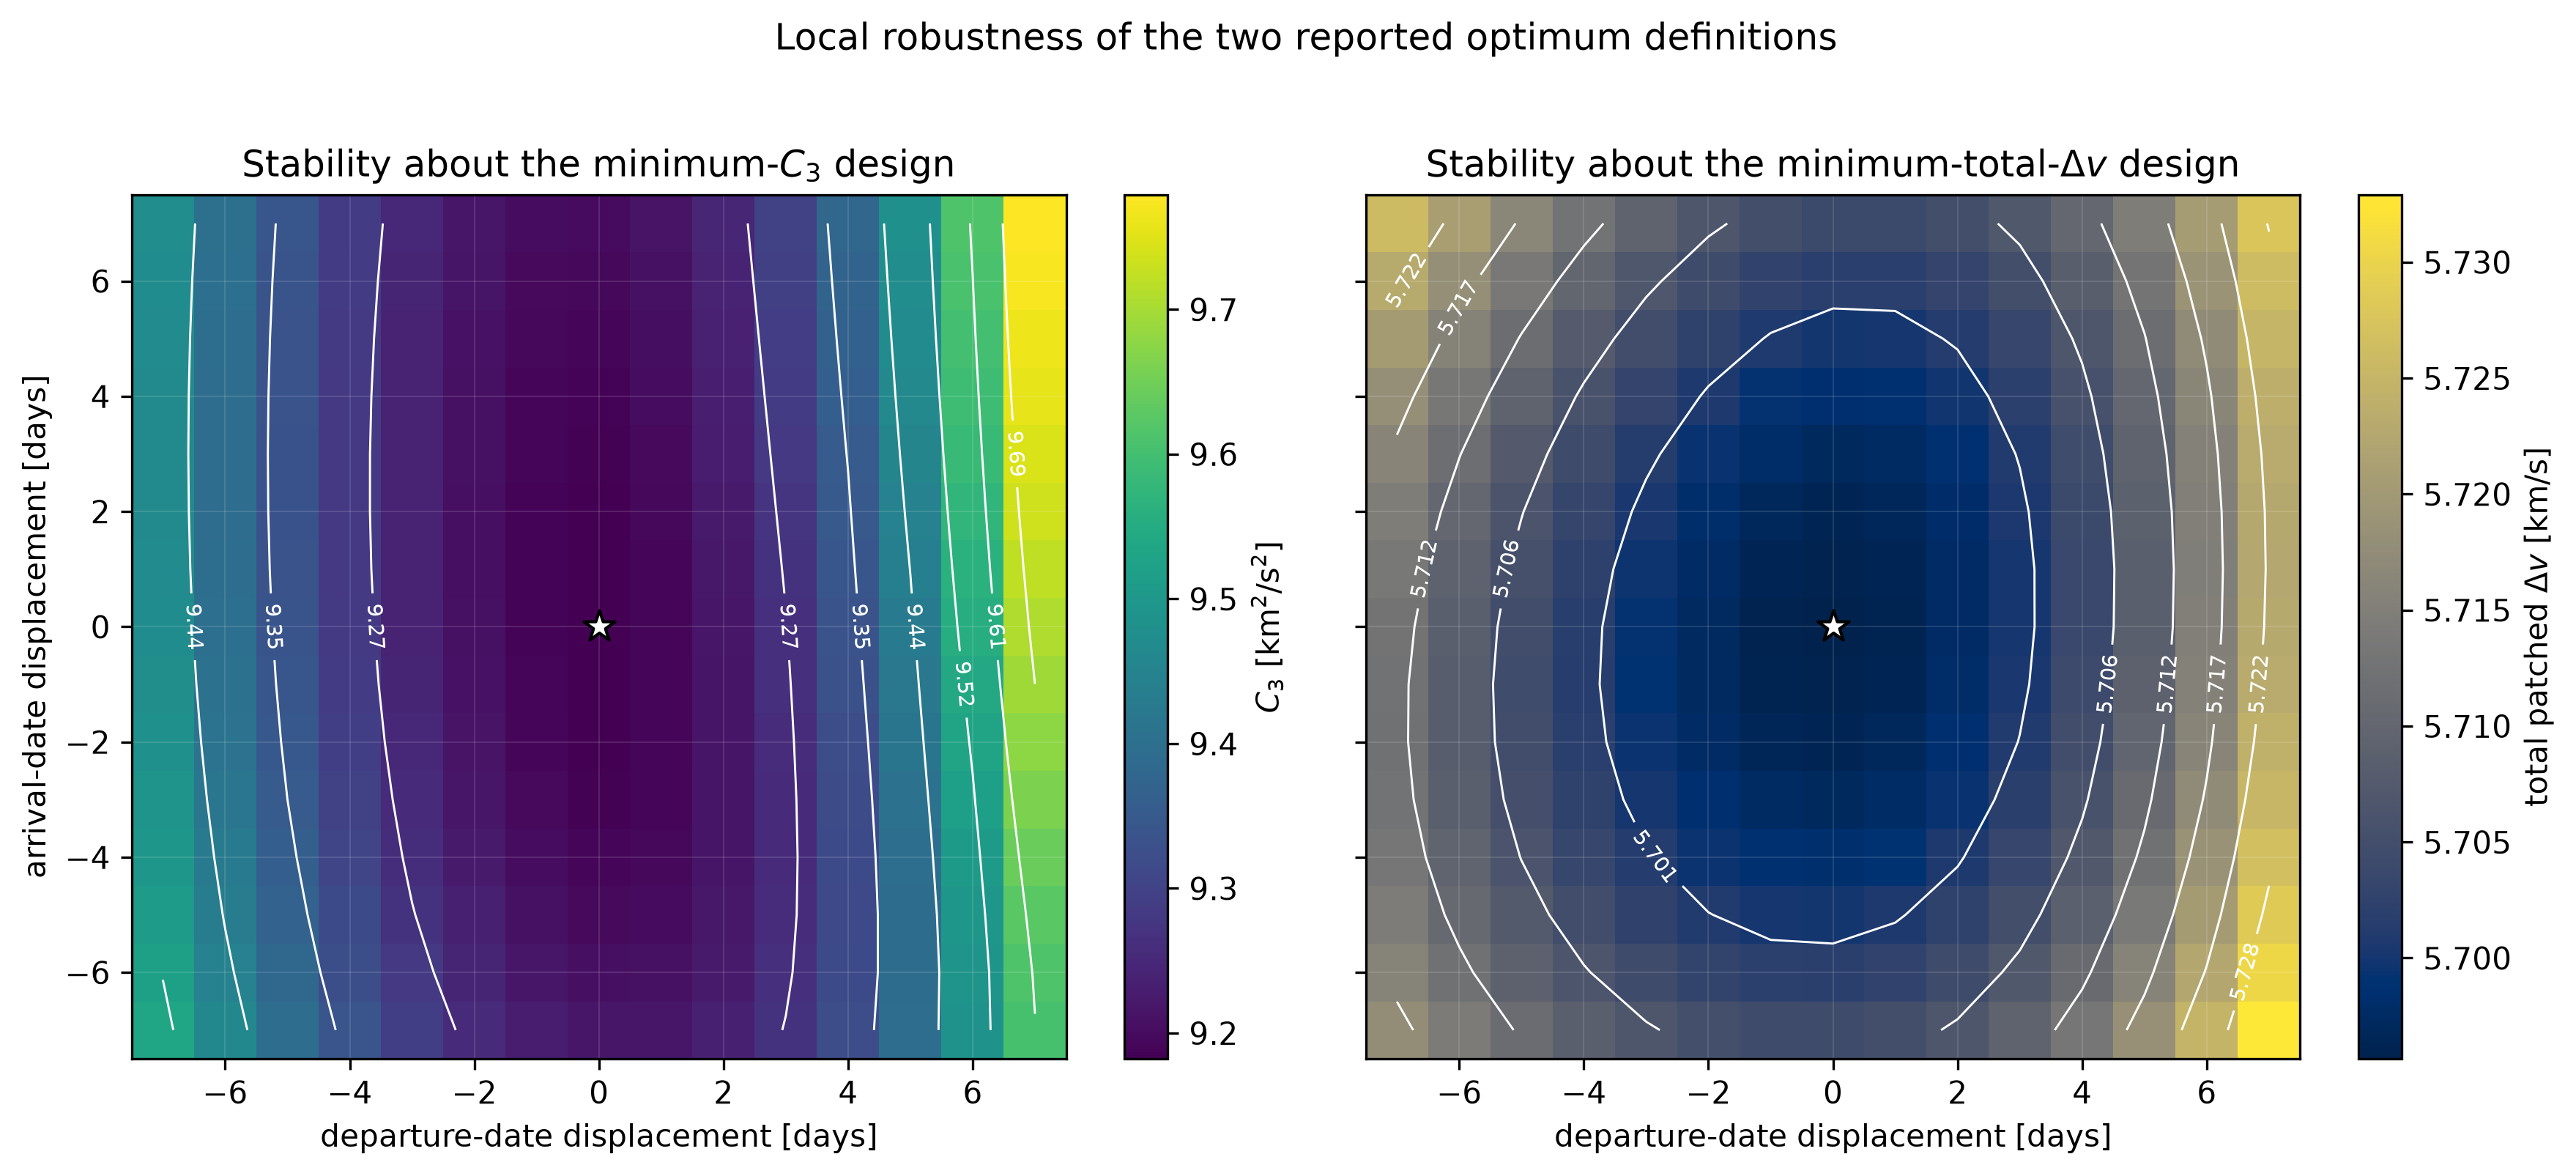
\includegraphics[width=\textwidth]{optimal_solution_stability.png}
  \caption{Local date sensitivity over independent $\pm7$ day perturbations of departure and arrival. Left: $C_3$ around the minimum-$C_3$ candidate. Right: total patched-conic $\Delta v$ around the minimum-total-$\Delta v$ candidate. The central star denotes the reported solution. Source: authors' calculations.}
  \label{fig:stability}
\end{figure}

The largest value increase in the displayed neighbourhood is approximately
$\CThreeStabilityWorstPenalty\,\mathrm{km^2\,s^{-2}}$ for the $C_3$ objective
and $\TotalDVStabilityWorstPenalty\,\mathrm{km\,s^{-1}}$ for the total-impulse
objective. Both candidates therefore lie in smooth low-cost regions rather
than at isolated numerical spikes.

\begin{figure}[H]
  \centering
  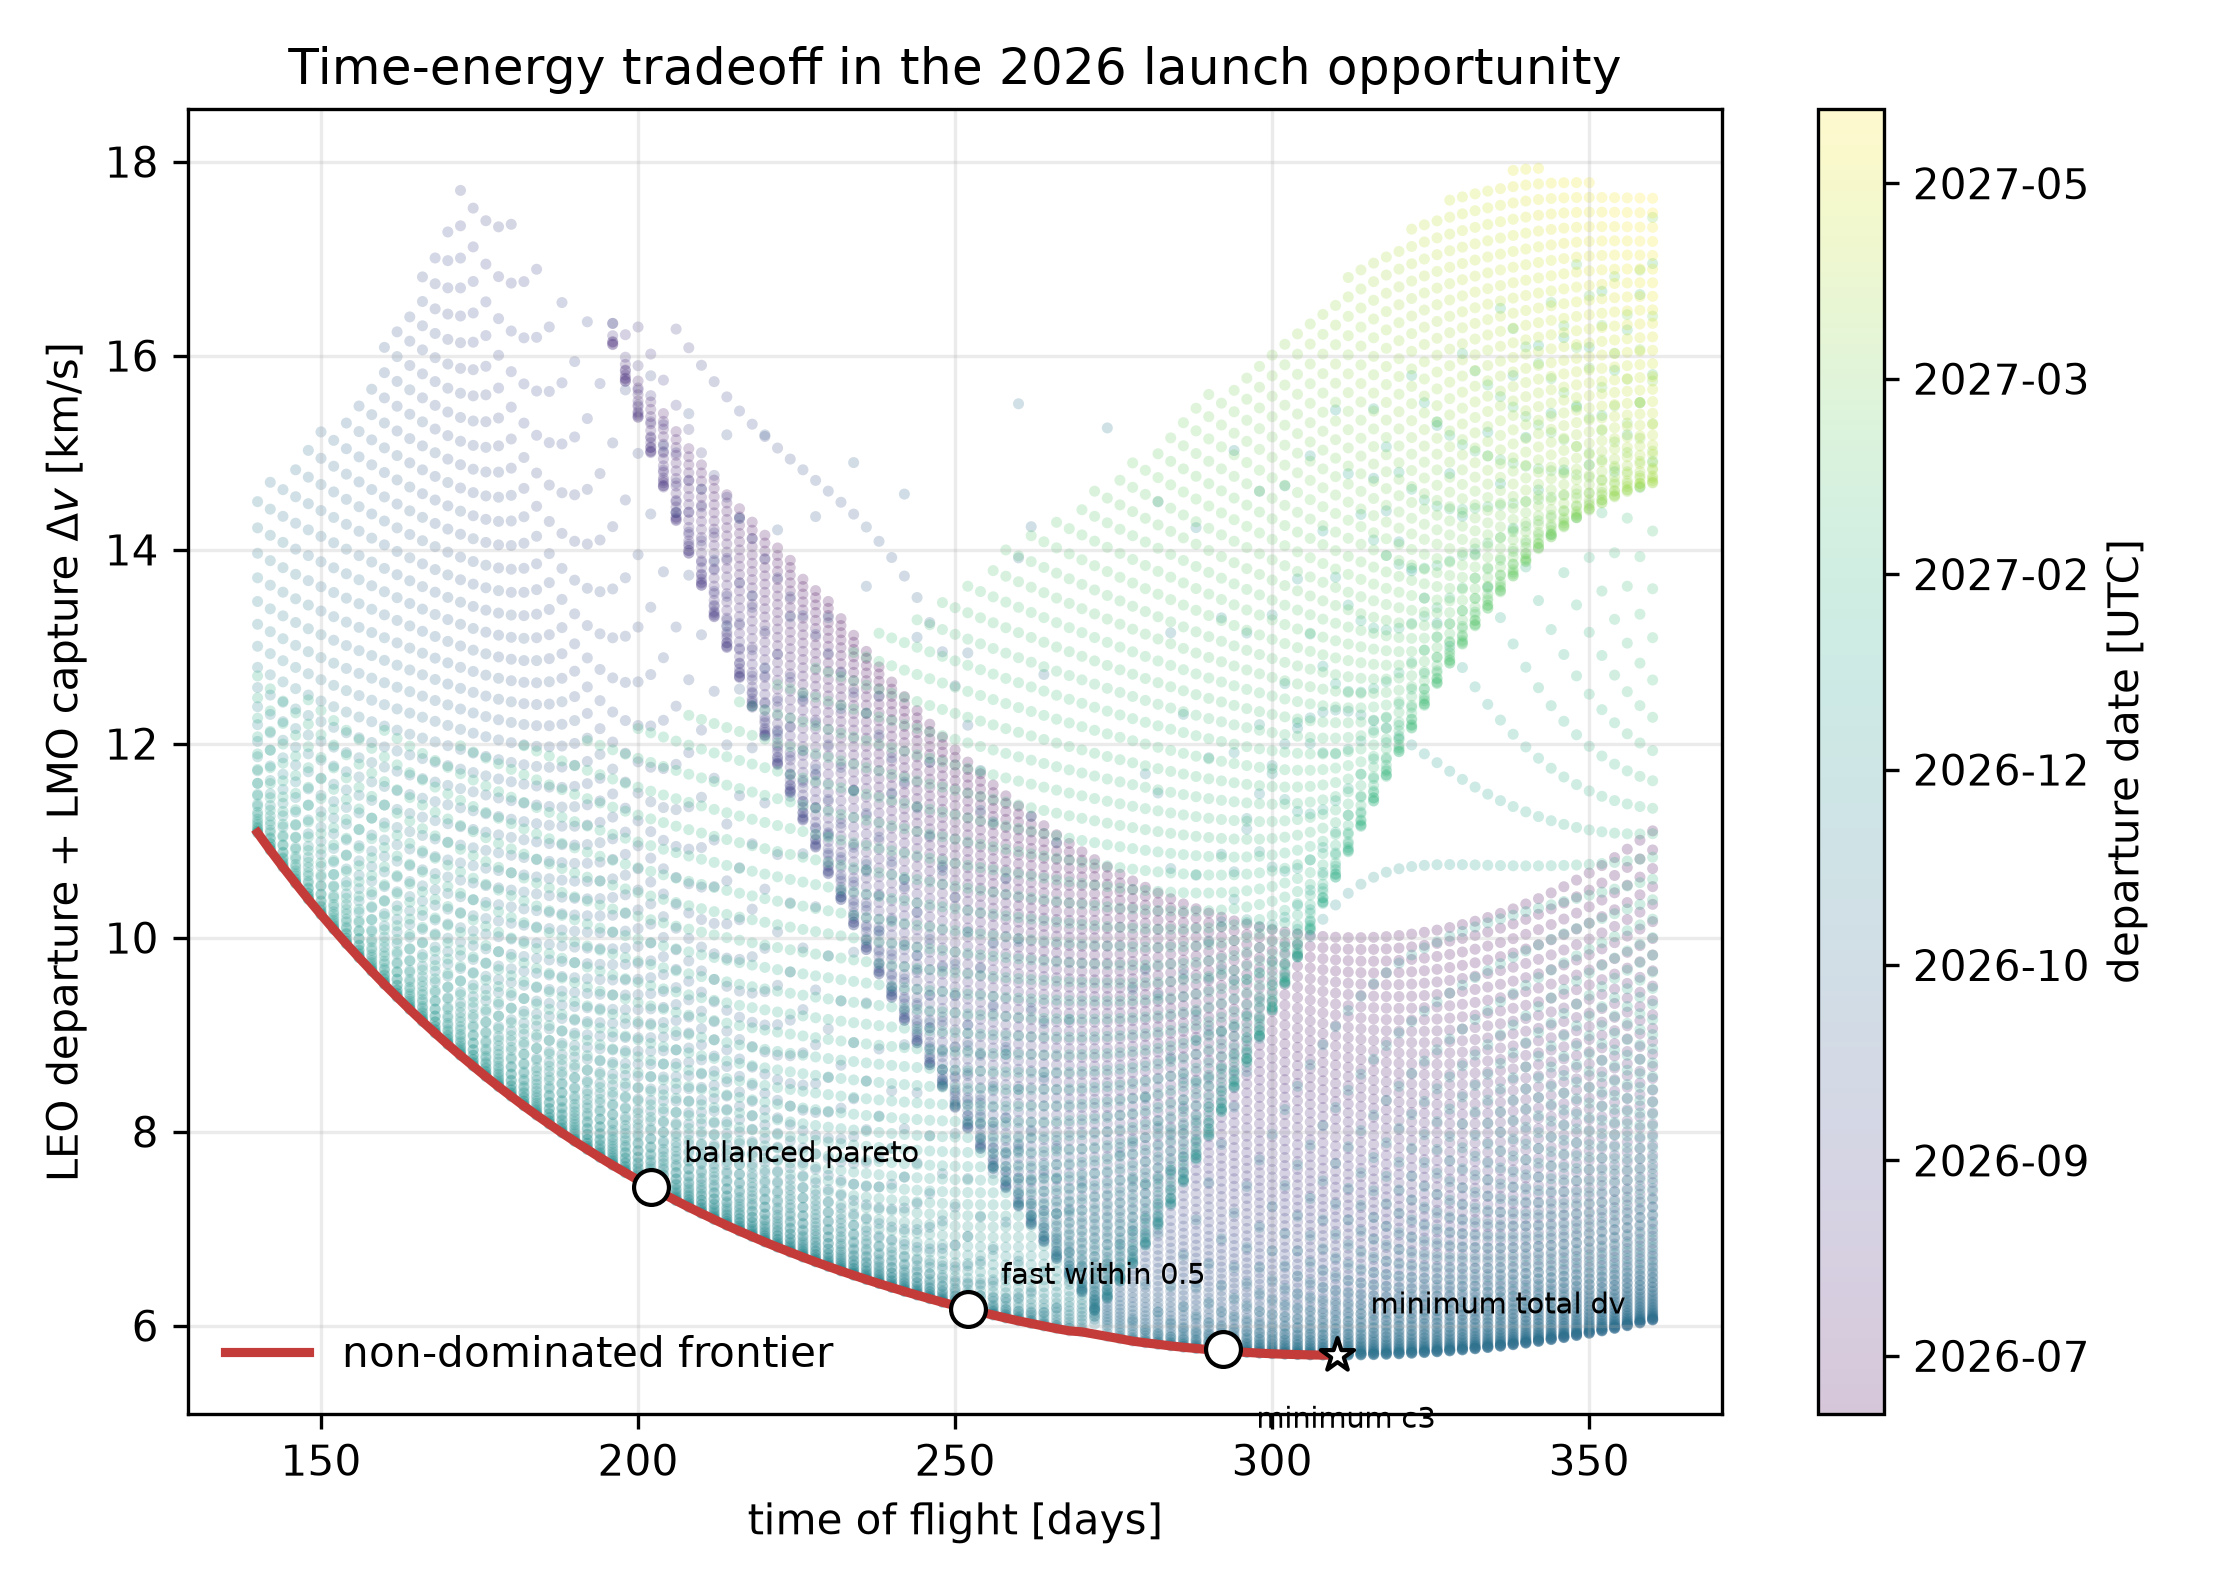
\includegraphics[width=0.80\textwidth]{pareto_time_delta_v.png}
  \caption{Time of flight versus the two-impulse patched-conic budget within the common analysis domain $v_{\infty,E}<12\,\mathrm{km\,s^{-1}}$ and $v_{\infty,M}<12\,\mathrm{km\,s^{-1}}$. The red curve is the strict nondominated frontier, the labelled symbols identify the same four designs reported in Table~\ref{tab:candidates}, and point colour represents departure date. Source: authors' calculations.}
  \label{fig:pareto}
\end{figure}

Figure~\ref{fig:pareto} provides the graphical counterpart of the four retained
selection rules. The minimum-total-$\Delta v$ and minimum-$C_3$ points occupy
the low-impulse end of the opportunity, the Fast (within 0.5 km/s) point accepts
a modest impulse increase for a shorter flight, and the balanced design lies
near the knee of the nondominated frontier. The figure therefore compares
mission preferences rather than claiming that one definition of ``optimal'' is
universally correct.

\subsection{Three-Dimensional Representation of the Recommended Trajectory}

Figure~\ref{fig:arc3d} visualizes the minimum-total-$\Delta v$ design retained
as the report's principal recommendation. The transfer is a prograde long-way
arc with transfer angle \MinimumTransferAngle{} degrees, heliocentric
semi-major axis \MinimumTransferSemimajor\AU{}, and transfer-plane inclination
\MinimumTransferInclination{} degrees relative to the J2000 ecliptic. Its Earth
departure characteristic energy is
$C_3=\MinimumCThree\,\mathrm{km^2\,s^{-2}}$, and its Martian arrival excess
speed is $\MinimumArrivalVInf\kms$.

\begin{figure}[H]
  \centering
  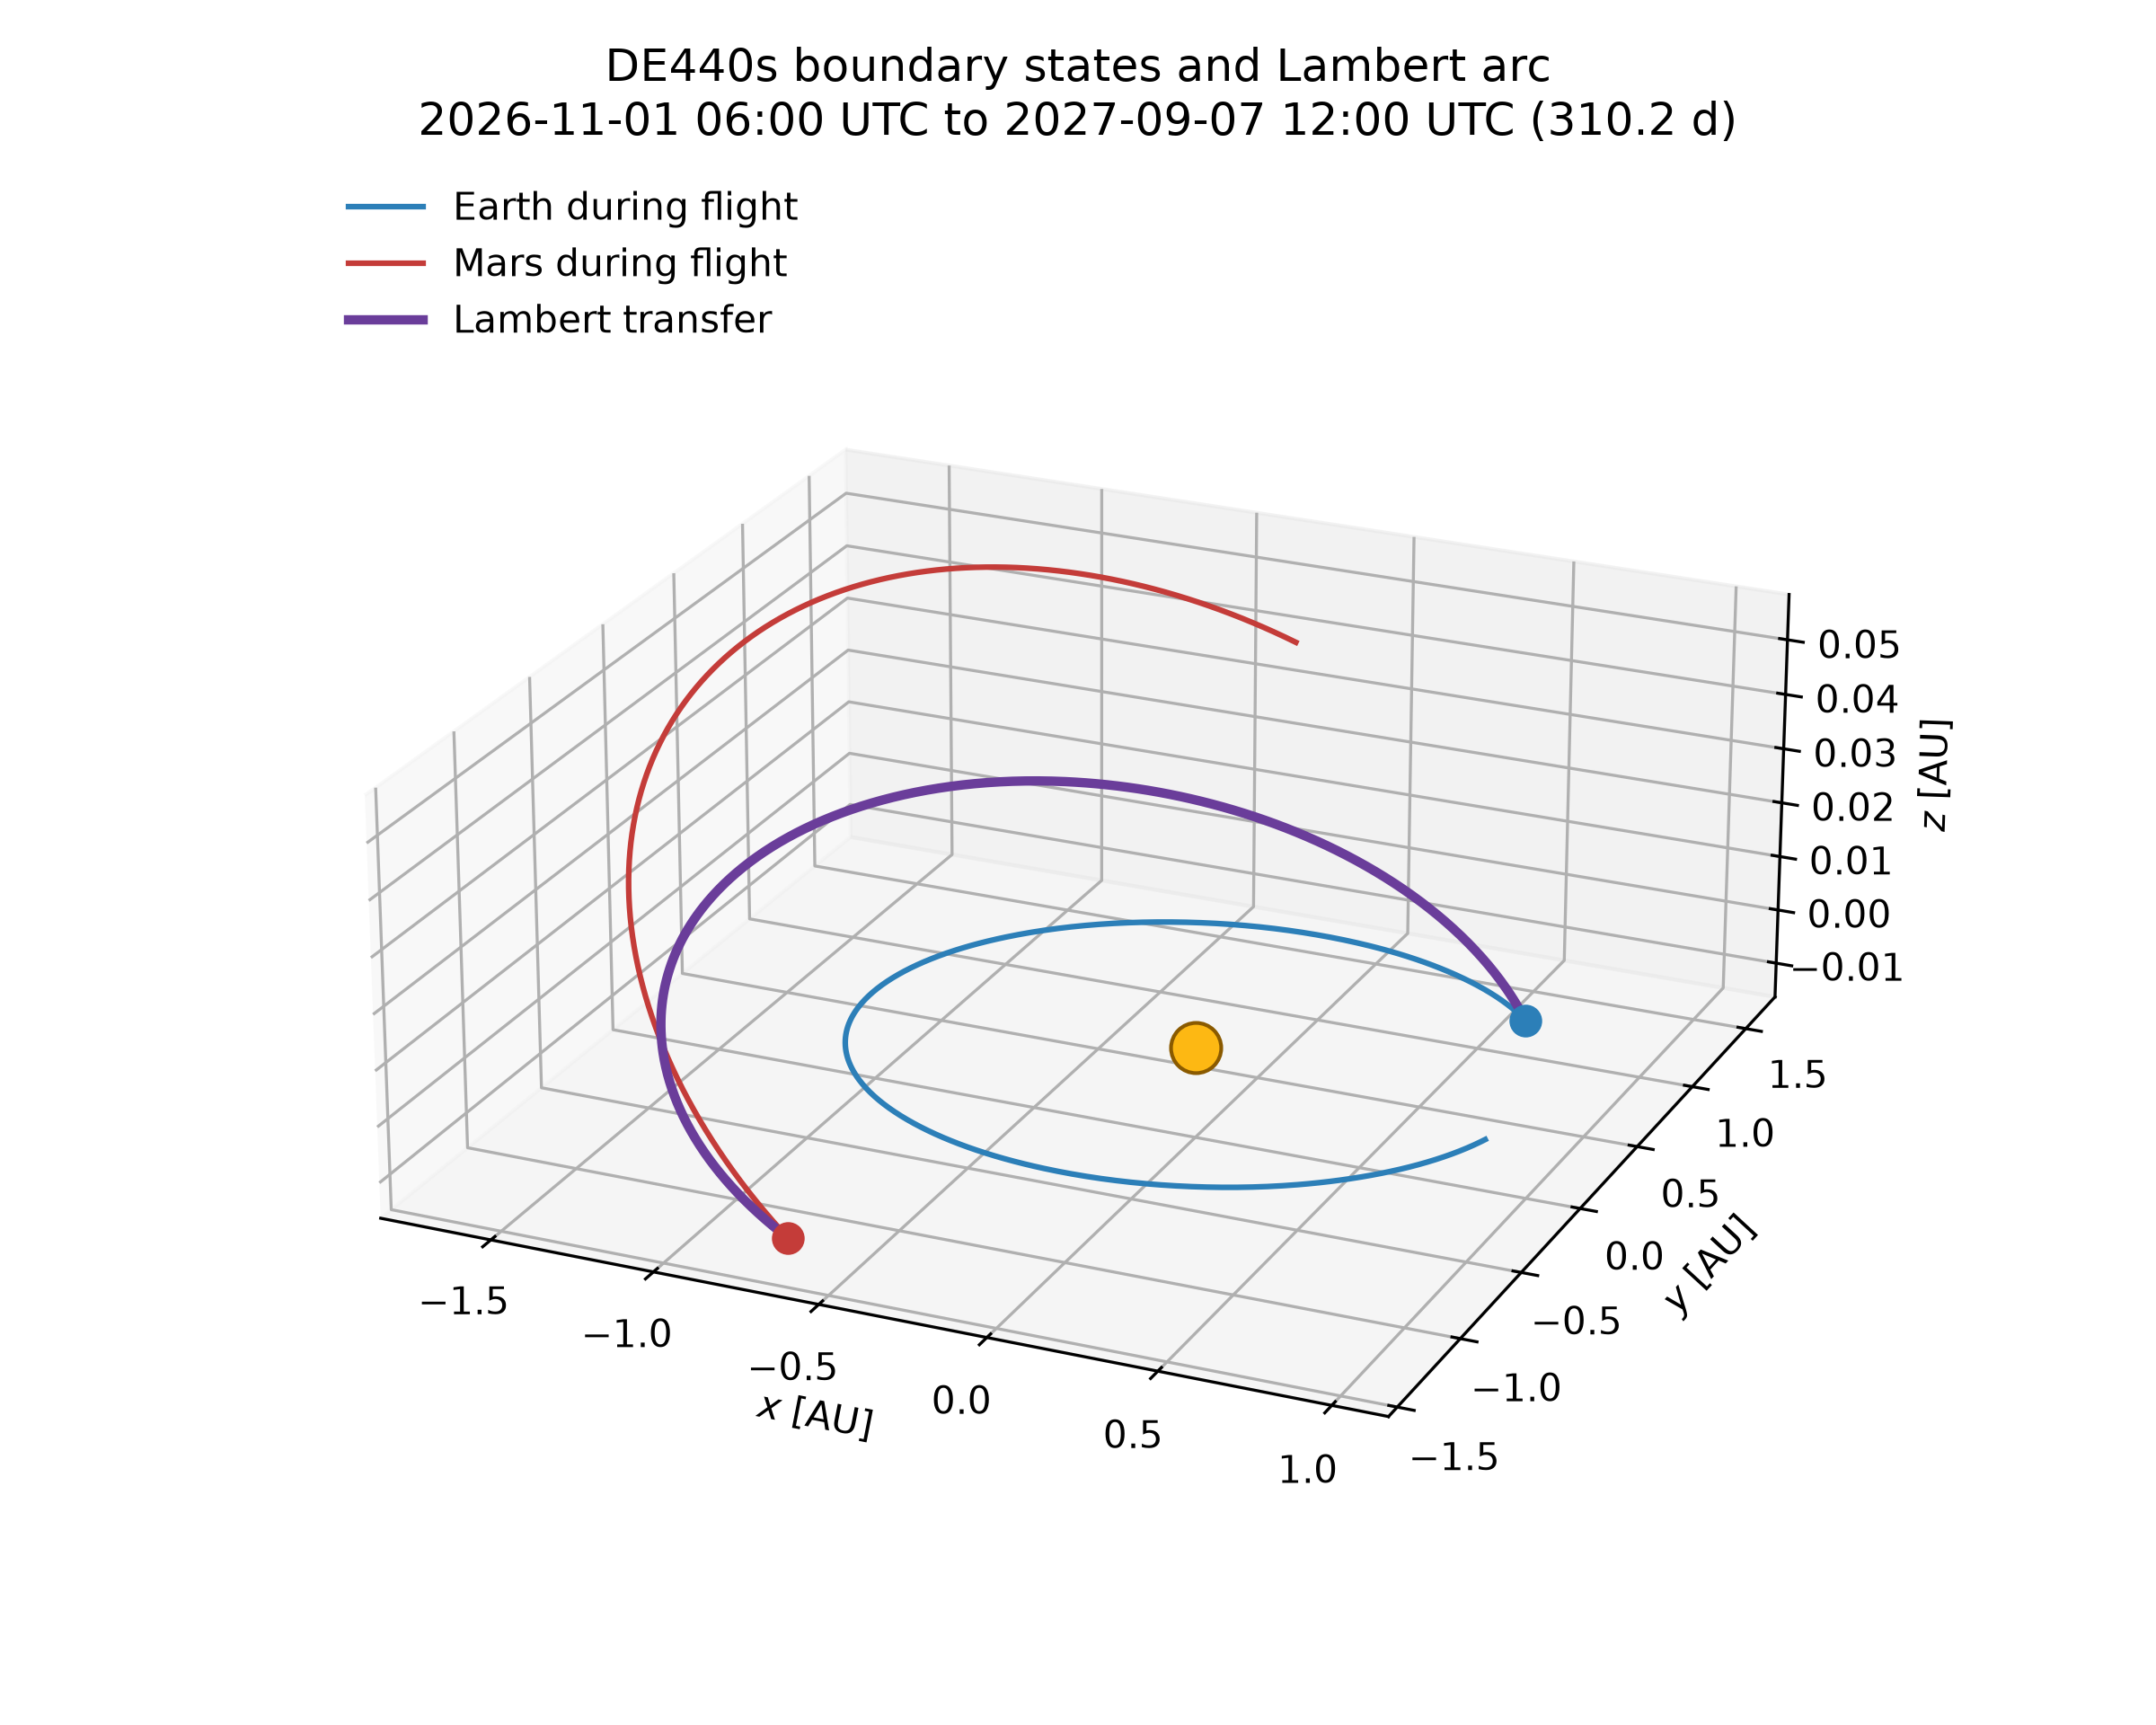
\includegraphics[width=0.82\textwidth]{lambert_transfer_3d.png}
  \caption{Three-dimensional Lambert transfer arc determined by the DE440s endpoint states for the minimum-total-$\Delta v$ design. The Earth and Mars curves show their motion during the transfer interval. All coordinate labels retain their numerical values in astronomical units, but the three-dimensional box uses a non-equal visual aspect so that the small out-of-ecliptic component remains visible; the plot should therefore be interpreted as a geometric visualization rather than an equal-scale measurement. Source: authors' calculations.}
  \label{fig:arc3d}
\end{figure}

The agreement among the Hohmann energy scale, the Standish screening model, and
the DE440s search supports the physical consistency of the selected launch
opportunity. The four-design framework then separates that numerical agreement
from the mission-level choice of objective. The remaining uncertainty is
dominated not by root-finding precision, but by model scope: a mission-design
continuation should propagate the four reported candidates in an $N$-body model
and then include launch-site, finite-burn, navigation, vehicle, and Mars-arrival
constraints.



\section{Gravity-Assist Theory and Sensitivity Analysis}
\label{sec:gravity-assist}

The Lambert problem provides a powerful framework for finding a Keplerian trajectory connecting two planetary states within a specified flight time. However, a Lambert solution only guarantees a dynamically feasible transfer; it does not necessarily minimize the propulsion requirement.

For interplanetary missions, reducing the required velocity increment
$\Delta v$ is a central design objective because launch mass and available fuel are strongly constrained. Therefore, modern mission designs often exploit the gravitational fields of other planets to modify the spacecraft trajectory without performing large propulsive maneuvers \cite{longuski1991}.

This technique is known as a \textit{slingshot manœuvres}, usually achieved through
a close planetary \textit{fly-by} maneuver.

\subsection{Hyperbolic Flyby Geometry}

\begin{figure}[H]
    \centering
    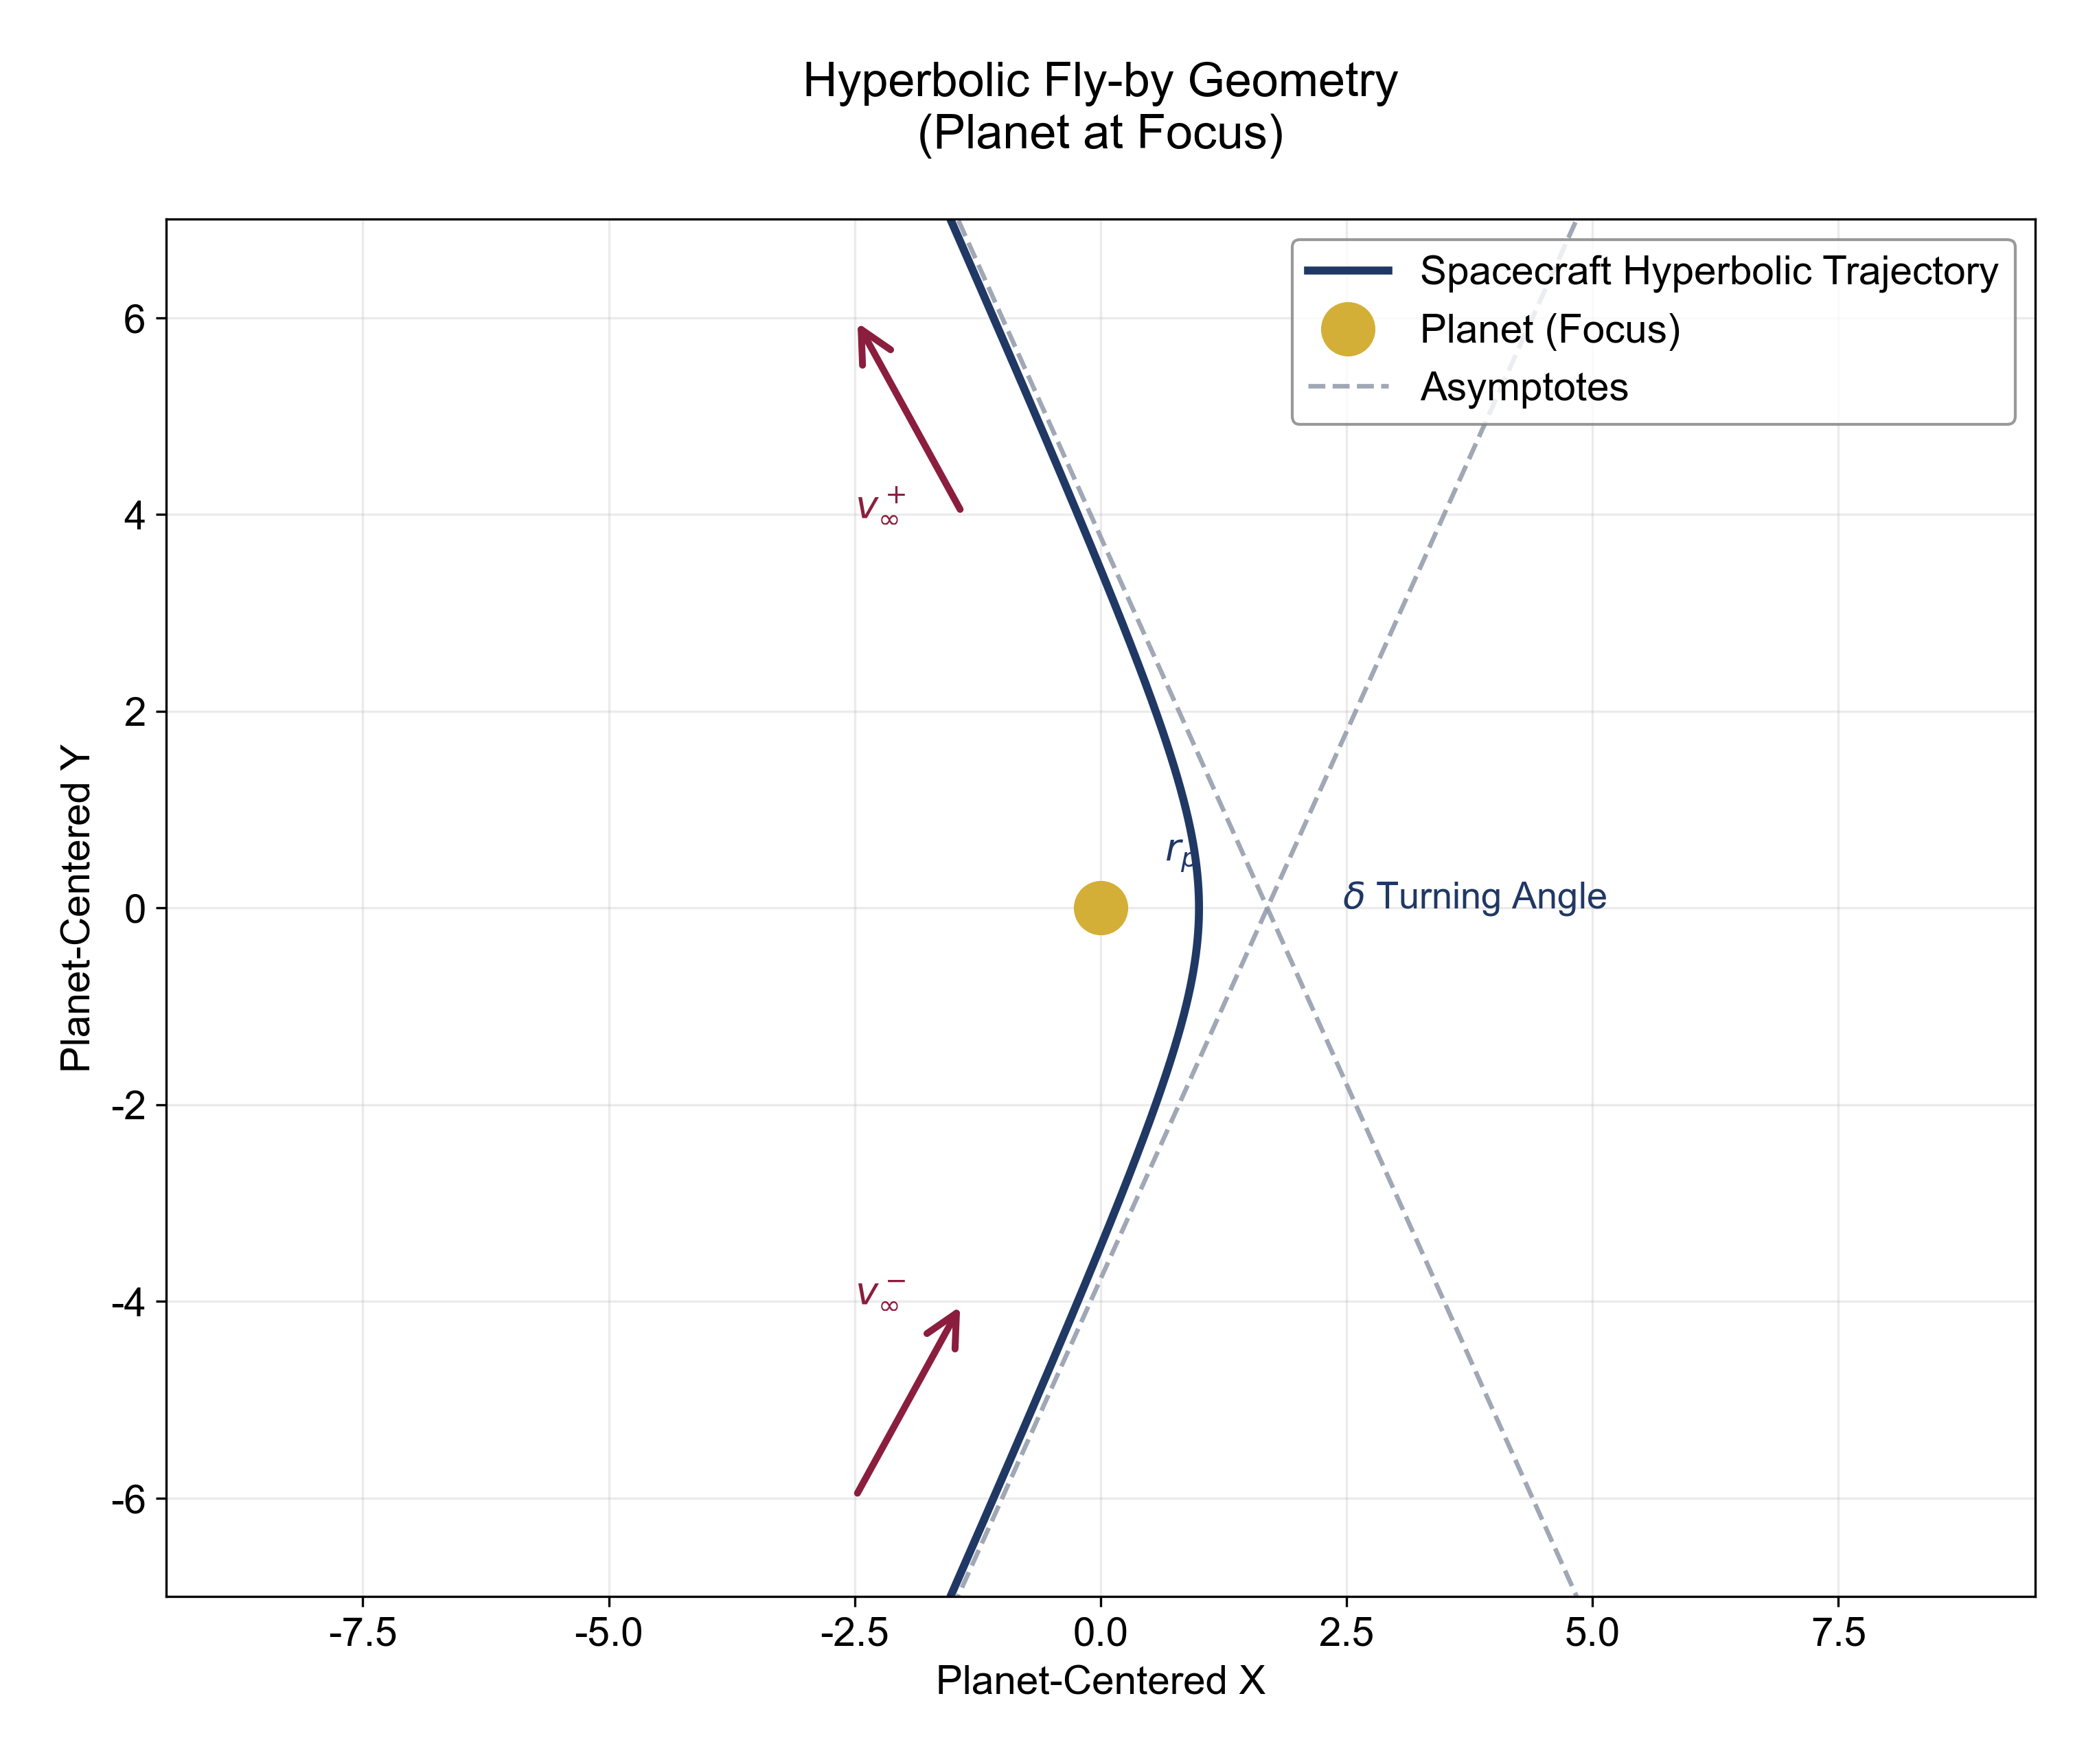
\includegraphics[width=0.85\textwidth]{fig3_flyby_hyperbola.png}
    \caption{Hyperbolic fly-by trajectory geometry in planet-centred inertial frame, labelling periapsis radius $r_p$, incoming/outgoing hyperbolic excess velocity $v_\infty^\pm$ and total deflection angle $\delta$.}
    \label{fig:hyper_geo}
\end{figure}

A fly-by maneuver occurs when a spacecraft passes close to a planet
without entering orbit or landing. It's speed will not be too large to be captured by the gravitational force of the target planet, which means that the trajrctory of the spacecraft is a hyperbola. During the encounter, the gravitational
attraction of the planet bends the spacecraft trajectory.

In the planet-centered reference frame, the spacecraft approaches the planet
with a hyperbolic excess velocity \cite{orbitalflyby}

\[
\mathbf{v}_{\infty}^{-},
\]

and leaves with

\[
\mathbf{v}_{\infty}^{+}.
\]

Here the hyperbolic excess velocity $v_\infty^{-}$ refers to the velocity of the aircraft when it is so far away from the planet that the gravitational force has little effect on it. We define it in this way to see the effect of the planet on the velocity of the air craft.

\[
\frac{1}{2}v^2 - \frac{\mu}{r} = \frac{1}{2}v_\infty^2,
\]
\[
\mu = GM.
\]

Because the gravitational interaction and the total energy is conservative, the magnitude of the hyperbolic excess velocity remains approximately unchanged:

\[
\left|\mathbf{v}_{\infty}^{-}\right|
=
\left|\mathbf{v}_{\infty}^{+}\right|
\]
in the planet-centered reference frame.

Therefore, the spacecraft does not gain kinetic energy in the planet-centered
frame. Instead, the main effect of the fly-by is a rotation of the velocity
vector.

The hyperbolic fly-by trajectory can be described by the orbit equation

\[
r=\frac{p}{1+e_h\cos\theta},
\]

where $p$ is the semi-latus rectum, $e_h$ is the eccentricity of the
hyperbolic trajectory, and $\theta$ is the true anomaly. For a hyperbolic
orbit,

\[
e_h>1.
\]

During a fly-by maneuver, the spacecraft moves along the asymptotic branches
of the hyperbolic trajectory when it is far away from the planet. Therefore,

\[
r\rightarrow\infty .
\]

For the orbit equation to approach infinity, the denominator must approach
zero:

\[
1+e_h\cos\theta_\infty=0.
\]

Therefore,

\[
\cos\theta_\infty=-\frac{1}{e_h}
\]

The asymptotic geometry of the hyperbolic trajectory determines the fly-by
turning angle. The turning angle $\delta$ is therefore related to the
eccentricity of the hyperbolic trajectory by

\[
\delta
=
\pm2\sin^{-1}
\left(
\frac{1}{e_h}
\right)
\]

where $e_h$ is the eccentricity of the spacecraft's trajectory
relative to the planet. The sign of $\delta$ is determined by the approaching direction. A smaller closest-approach distance produces a larger
turning angle and therefore a greater modification of the heliocentric
trajectory.


\subsection{Reference-Frame Interpretation of Energy Exchange}

Although the spacecraft speed relative to the planet remains almost unchanged,
the situation is different in the heliocentric reference frame \cite{curtis2020}.

Let the velocity of the planet around the Sun be

\[
\mathbf{v}_p.
\]

The spacecraft heliocentric velocities before and after the encounter are

\[
\mathbf{v}_{before}
=
\mathbf{v}_p+\mathbf{v}_{\infty}^{-},
\]

and

\[
\mathbf{v}_{after}
=
\mathbf{v}_p+\mathbf{v}_{\infty}^{+}.
\]

Since the direction of $\mathbf{v}_{\infty}$ changes during the fly-by, the
magnitude of the spacecraft heliocentric velocity can increase or decrease, depending on the approaching direction of the aircraft.

For an accelerating gravity assist,

\[
|\mathbf{v}_{after}|
>
|\mathbf{v}_{before}|,
\]

the spacecraft gains heliocentric orbital energy. Conversely, a decelerating
fly-by satisfies

\[
|\mathbf{v}_{after}|
<
|\mathbf{v}_{before}|.
\]

The additional energy obtained by the spacecraft is not created
spontaneously. It is transferred from the orbital energy of the planet. Since
the mass of the planet is many orders of magnitude larger than the spacecraft
mass, the corresponding change in the planet's orbit is negligible.

%%%%%%%%%%%%%%%%%%%%%%%%%%%%%%%%%%%%%%%%%%%%%%%%%%%%%%%%%%%%
\subsection{Numerical Reconstruction of a Jupiter Gravity Assist}

The analytical flyby model developed in Sections~6.1 and~6.2 is validated through the reconstruction of the Voyager~1 Jupiter encounter. Rather than introducing additional theoretical derivations, the previously established hyperbolic flyby equations are applied directly to representative mission data. This example demonstrates how the analytical model predicts the turning angle and velocity-vector change produced by a practical gravity-assist maneuver.

Voyager~1 is selected because Jupiter possesses the largest gravitational parameter and sphere of influence among the planets, making it the most effective body for gravity-assist trajectory design \cite{curtis2020}. The encounter parameters were compiled from the NASA Voyager mission archive and the JPL DE440 planetary ephemeris.

The encounter parameters were compiled from the NASA Voyager mission archive \cite{voyager1} and the JPL DE440 planetary ephemeris \cite{park2021}.

The adopted planetary constants are

\begin{itemize}
    \item Jupiter gravitational parameter
    \[
        \mu_{\rm J}=126\,712\,764.1\ {\rm km^3\,s^{-2}} ( \cite{park2021})
    \]

    \item Jupiter mean radius
    \[
        R_{\rm J}=71\,492\ {\rm km}
    \]

    \item Jupiter heliocentric orbital velocity
    \[
        V_{\rm J}=13.07\ {\rm km\,s^{-1}}
    \]
\end{itemize}

For the Voyager~1 flyby, the adopted encounter conditions are

\begin{itemize}
    \item Hyperbolic excess velocity
    \[
        v_\infty=10.8\ {\rm km\,s^{-1}}
    \]

    \item Closest approach altitude
    \[
        h=280\,000\ {\rm km}
    \]
\end{itemize}

The periapsis radius is therefore

\begin{align}
r_p
&=R_{\rm J}+h
\nonumber\\
&=71\,492+277\,400
\nonumber\\
&=348\,892\ {\rm km}.
\end{align}

Using the analytical model,

\begin{align}
a
&=-\frac{\mu_{\rm J}}{v_\infty^2}
\nonumber\\
&=-\frac{126,712,764.1}{10.8^2}
\nonumber\\
&=-1\,086\,358\ {\rm km},
\\[0.25cm]
e
&=1+\frac{r_pv_\infty^2}{\mu_{\rm J}}
\nonumber\\
&=1+\frac{348\,892\times10.8^2}
{126,712,764.1}
\nonumber\\
&=1.321,
\\[0.25cm]
\delta
&=2\arcsin\!\left(\frac1e\right)
\nonumber\\
&=98.4^\circ,
\\[0.25cm]
\Delta v_{\max}
&=2v_\infty
\sin\!\left(\frac{\delta}{2}\right)
\nonumber\\
&=16.35\ {\rm km\,s^{-1}}.
\end{align}

The reconstructed encounter yields a turning angle close to $100^\circ$, indicating substantial gravitational bending of the incoming trajectory. While the spacecraft speed relative to Jupiter remains constant throughout the flyby, the direction of the hyperbolic excess velocity vector changes significantly. This rotation enables the exchange of orbital energy in the heliocentric reference frame without consuming onboard propellant. The reconstructed results agree with the expected characteristics of the Voyager~1 Jupiter encounter and provide numerical validation of the analytical gravity-assist model developed in this chapter.

\begin{figure}[H]
    \centering
    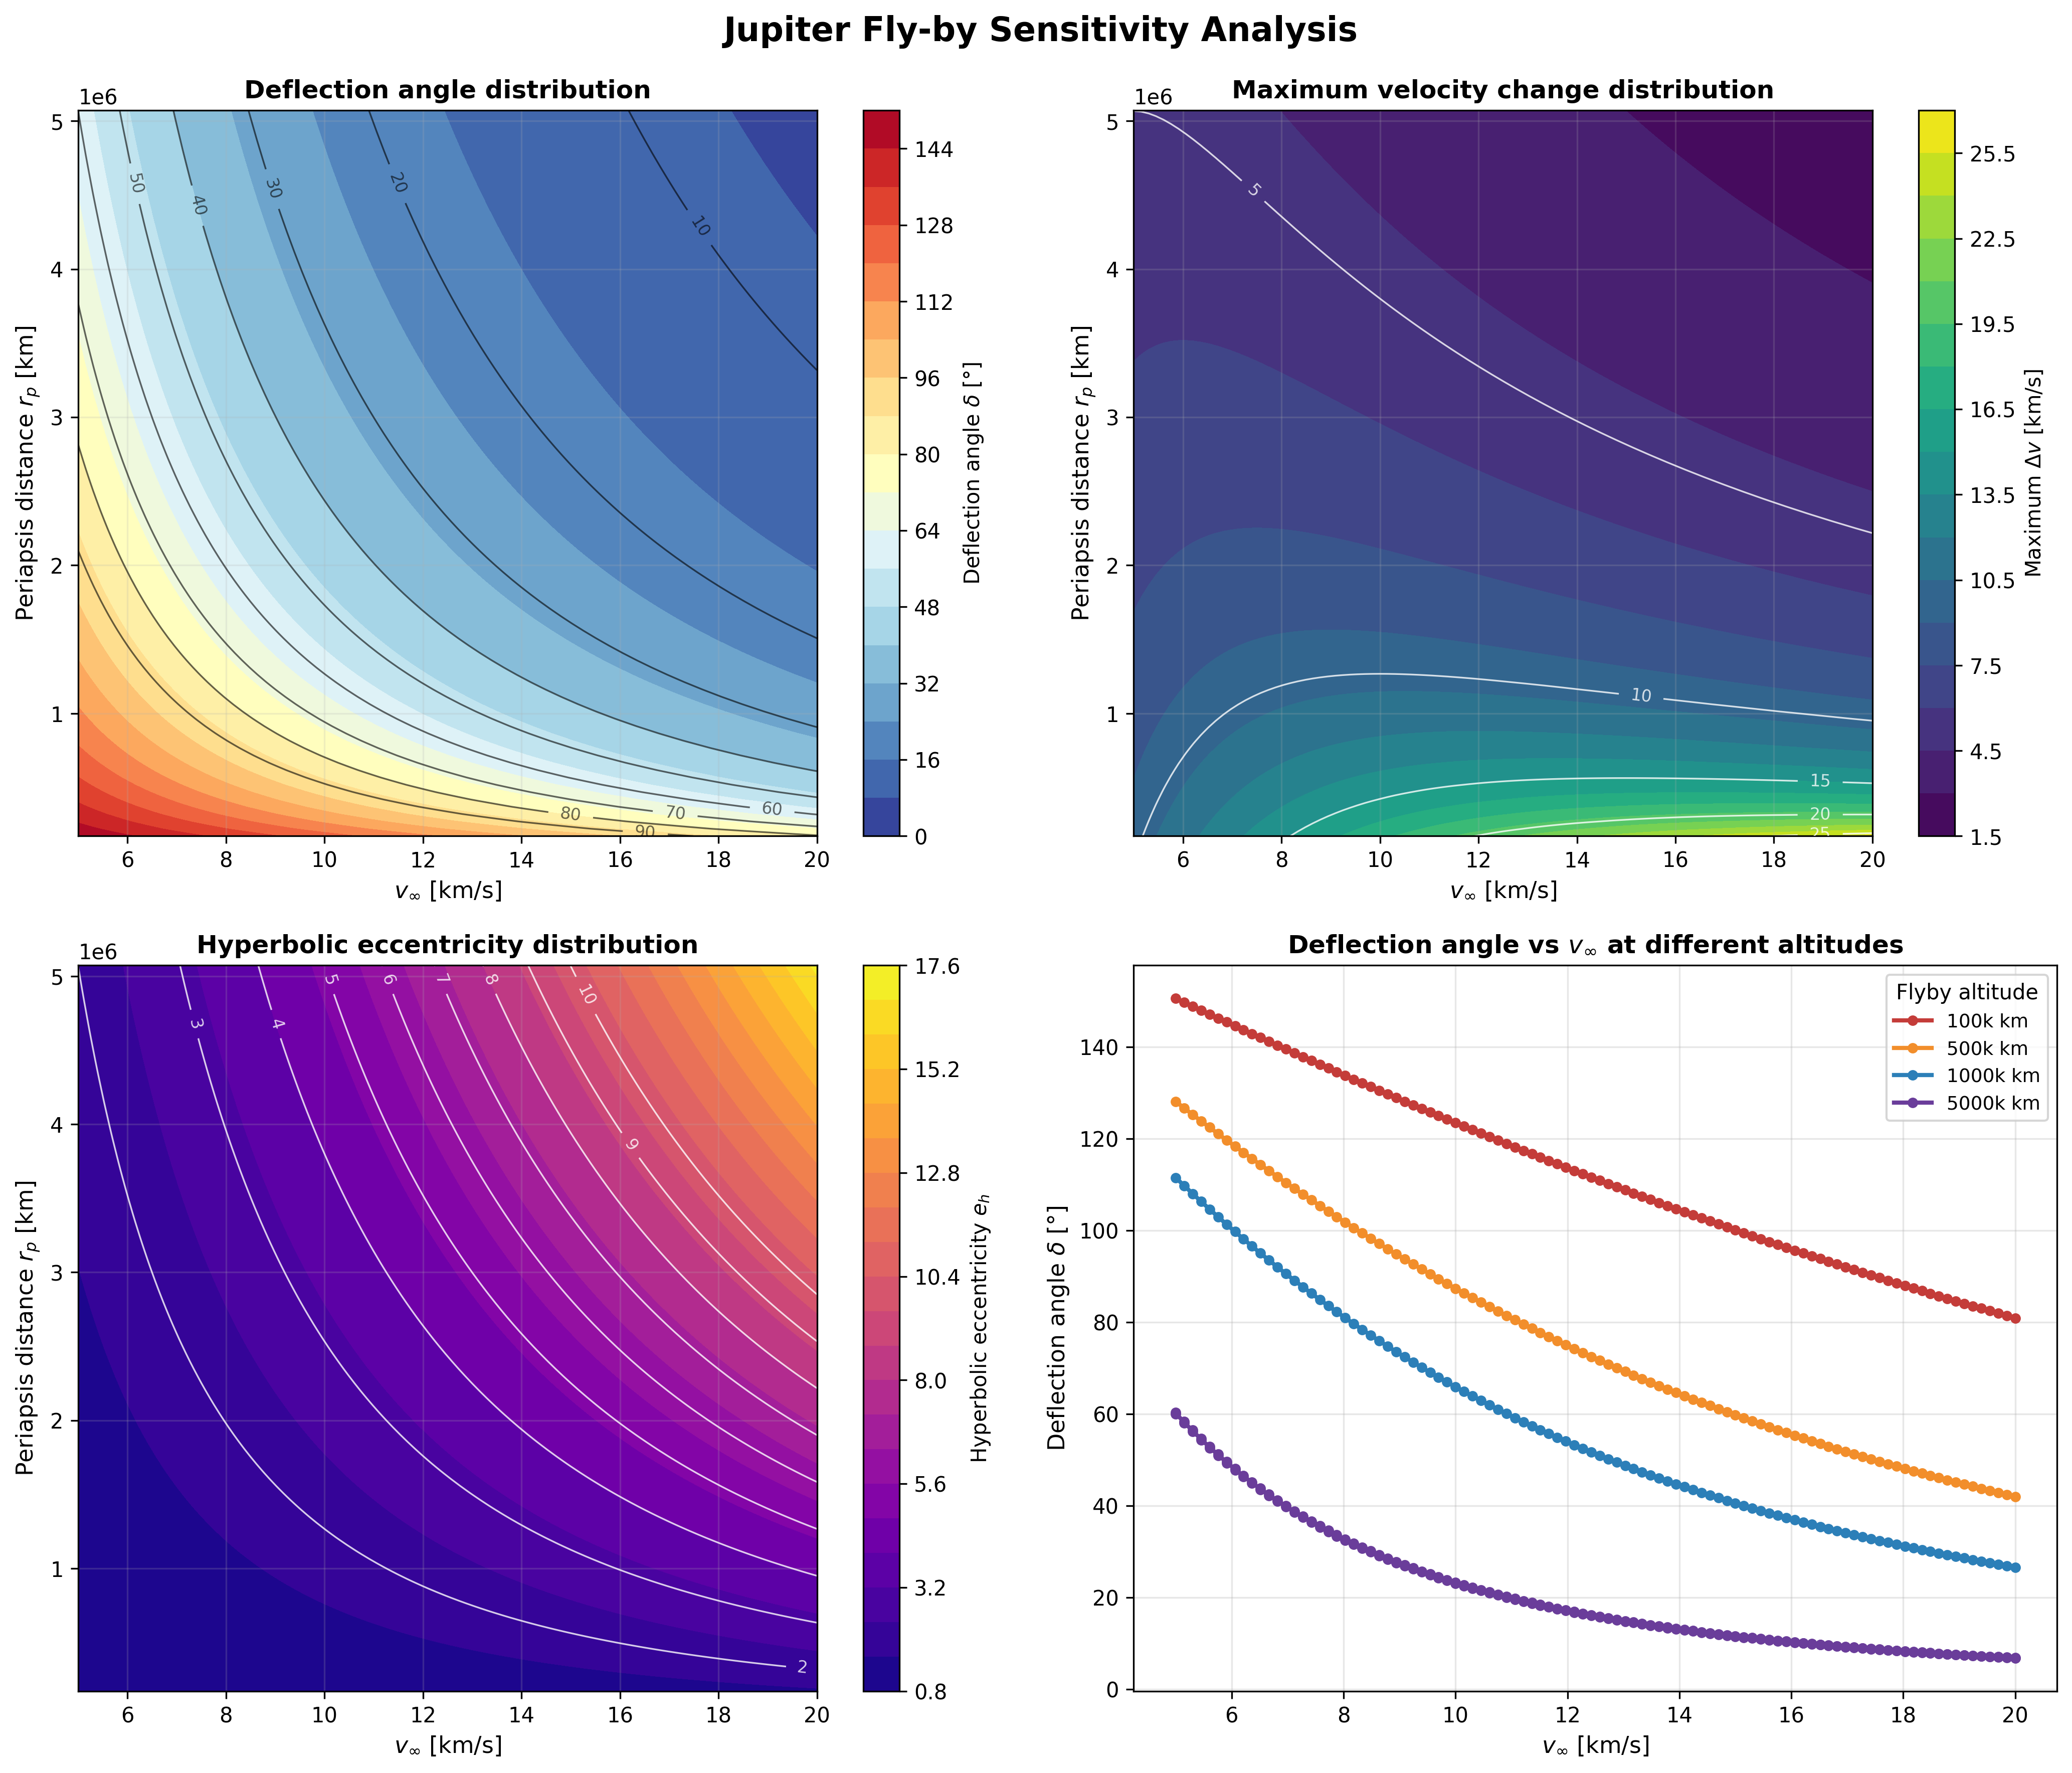
\includegraphics[width=0.90\textwidth]{jupiter_sensitivity_analysis.png}
    \caption{Parametric contour plots of core fly-by quantities as functions of hyperbolic excess speed $v_\infty$ and periapsis altitude: top-left total deflection angle $\delta$ (°), top-right maximum achievable $\Delta v_{\max}$ ($\mathrm{km\,s^{-1}}$), bottom-left hyperbolic eccentricity $e_h$, bottom-right peak $\Delta v$ trend curves for fixed periapsis radii (100/500/1000/5000 km). Source: Author's calculation}
    \label{fig:flyby_param_contours}
\end{figure}

%%%%%%%%%%%%%%%%%%%%%%%%%%%%%%%%%%%%%%%%%%%%%%%%%%%%%%%%%%%%
\subsection{Sensitivity Analysis}

The analytical model also enables a systematic investigation of how the principal flyby parameters vary with encounter geometry. Figure~\ref{fig:flyby_param_contours} presents the numerical results obtained by varying the hyperbolic excess velocity and periapsis altitude while keeping the planetary gravitational parameter fixed at that of Jupiter. These contour maps provide a direct visualization of the relationships among flyby altitude, incoming velocity, trajectory deflection and the achievable velocity-vector change.

The upper-left panel shows that decreasing periapsis altitude increases the turning angle because the spacecraft experiences stronger gravitational bending. Conversely, larger hyperbolic excess velocities shorten the interaction time within the planet's sphere of influence, producing smaller trajectory deflections. Therefore, large turning angles are obtained primarily during low-altitude, low-velocity flybys.

The upper-right panel illustrates the variation of the theoretical maximum velocity-vector change. Although increasing $v_\infty$ reduces the turning angle, it simultaneously increases the velocity magnitude. As a result, the maximum achievable $\Delta v$ depends on the combined influence of both parameters rather than either one individually.

The lower-left panel confirms the inverse relationship between eccentricity and turning angle predicted by the analytical expression, while the lower-right panel shows that lower flyby altitudes consistently produce larger velocity-vector changes.

The lower-right panel compares the variation of $\Delta v_{\max}$ for several representative periapsis altitudes. At low flyby altitudes the velocity-vector change increases rapidly before gradually approaching a plateau as $v_\infty$ increases. Higher-altitude flybys produce consistently smaller values of $\Delta v_{\max}$ over the entire velocity range because the weaker gravitational interaction limits the achievable trajectory rotation \cite{bate1971}.

These results indicate a fundamental engineering trade-off. Lower-altitude flybys provide greater gravity-assist efficiency but require higher navigation accuracy, whereas higher-altitude encounters are operationally safer at the expense of reduced trajectory modification.

%%%%%%%%%%%%%%%%%%%%%%%%%%%%%%%%%%%%%%%%%%%%%%%%%%%%%%%%%%%%
\subsection{Comparative Mission Analysis}

To further evaluate the analytical model, representative gravity-assist missions involving both inner and outer planets were reconstructed using the same calculation procedure. The resulting encounter parameters are summarized in Table~\ref{tab:flyby_results}.

\begin{table}[H]
  \centering
   \caption{Gravity-assist mission parameters and calculated flyby results. Encounter parameters were compiled from NASA/ESA mission archives and JPL DE440 ephemerides, while the turning angles and theoretical velocity-vector changes were calculated using the analytical model developed in this work.}
  \label{tab:flyby_results}
  \small
  \begin{tabular}{lccccc}
    \toprule
    Mission & Planet & $v_\infty$ [km/s] & $Altitude$ [km] & $\delta$ [°] & $\Delta v_{max}$ [km/s] \\
    \midrule
    Voyager 1 & Jupiter & 10.8 & 277,400 & 98.4 & 16.35 \\
    Voyager 2 & Jupiter & 13.6 & 720,000 & 55.3 & 12.62 \\
    Voyager 2 & Saturn & 10.5 & 101,000 & 85.8 & 14.30 \\
    Galileo & Earth & 8.9 & 300 & 50.9 & 7.65 \\
    Cassini & Venus & 7.2 & 284 & 59.6 & 7.16 \\
    New Horizons & Jupiter & 18.0 & 2,304,537 & 16.2 & 5.09 \\
    Rosetta & Earth & 2.6 & 2,481 & 120.8 & 4.52 \\
    MESSENGER & Mercury & 4.9 & 200 & 29.9 & 2.53 \\
    \bottomrule
  \end{tabular}
\end{table}

Figure~\ref{fig:mission_bar} presents a visual comparison of the turning angle and theoretical maximum velocity-vector change for the selected gravity-assist missions.

\begin{figure}[H]
    \centering
    
\includegraphics[width=0.85\textwidth]{figures/historical_mission_comparison.png}
   \caption{Comparison of representative gravity-    assist missions. Flyby encounter parameters (mission dates, flyby    planets, periapsis altitudes and hyperbolic excess velocities) 
    were compiled from NASA/ESA mission archives and JPL DE440 ephemerides. Turning angles and theoretical velocity-vector changes were calculated using the analytical model developed 
in this work. Source: authors’ calculations.}
    \label{fig:mission_bar}
\end{figure}

The comparison reveals several trends consistent with the sensitivity analysis. Giant planets such as Jupiter and Saturn generate the largest velocity-vector changes because of their strong gravitational fields and high orbital velocities, as demonstrated by the Voyager missions \cite{voyager1}. In contrast, terrestrial planets generally produce smaller velocity changes but can achieve relatively large turning angles when the incoming hyperbolic excess velocity is low. For example, the Rosetta Earth flyby exhibits the largest turning angle in Table~\ref{tab:flyby_results}, whereas the New Horizons Jupiter encounter shows that even a distant flyby can provide a useful trajectory modification when the incoming velocity is sufficiently high.

Overall, the agreement between the reconstructed mission parameters and the theoretical trends observed in the sensitivity analysis demonstrates that the proposed flyby model successfully captures the principal characteristics governing practical gravity-assist trajectory design.

%%%%%%%%%%%%%%%%%%%%%%%%%%%%%%%%%%%%%%%%%%%%%%%%%%%%%%%%%%%%
\subsection{Engineering Implications}

The analytical model, sensitivity analysis and reconstructed mission examples demonstrate that gravity-assist trajectory design depends on the combined effects of planetary mass, encounter geometry and hyperbolic excess velocity. Effective trajectory design therefore requires balancing trajectory deflection, velocity-vector change and operational constraints rather than maximizing a single parameter.

Close flybys generally provide larger trajectory deflections but require greater navigation accuracy, whereas higher-altitude encounters are operationally safer at the expense of reduced gravity-assist efficiency \cite{strange2002}. Likewise, giant planets are better suited for major energy transfer, while terrestrial planets are more useful for trajectory correction and orbital adjustment.

These observations also explain why modern deep-space missions frequently employ multiple gravity assists rather than relying on a single planetary encounter. Each flyby contributes a partial modification of the spacecraft trajectory, allowing orbital energy and flight geometry to be adjusted progressively while remaining within the capability of existing launch vehicles. The cumulative effect of several moderate gravity assists often provides greater mission flexibility than attempting to maximize the performance of an individual flyby.

These characteristics explain why modern interplanetary missions often employ multiple gravity assists. Successive flybys allow orbital energy and trajectory geometry to be modified progressively, providing greater flexibility than relying on a single encounter.

Although this study focuses on Earth--Mars transfer analysis, the analytical framework developed here can be readily extended to multi-leg interplanetary trajectories involving additional planetary flybys. The consistency between theoretical predictions, sensitivity analysis and representative mission data demonstrates that the proposed model provides a reliable foundation for preliminary gravity-assist trajectory design.

\section{Model Validation, Limitations, and Further Work}
\label{sec:validation-limitations}

\subsection{Internal Numerical Checks}

Each Lambert solution is checked by propagating the computed departure state
through the same two-body model and comparing the propagated endpoint with the
prescribed arrival position. The reported endpoint residual is approximately
\LambertEndpointError{} km. Local perturbations of the departure and arrival
dates also show that the selected candidates lie in smooth low-cost regions
rather than at isolated numerical artifacts.

\subsection{Scope and Limitations}

The date-specific transfer analysis combines DE440s planetary boundary states
with a Sun--spacecraft two-body Lambert arc, impulsive maneuvers, and
patched-conic departure and capture estimates. It does not include finite-burn
dynamics, launch-site geometry, spacecraft mass ratios, atmospheric entry,
midcourse correction budgets, or full multi-body perturbations. The historical
flyby calculations are simplified illustrative two-body reconstructions rather than
navigation-grade reproductions of the original missions.

\subsection{Further Development}

A higher-fidelity extension would compare independent Lambert algorithms,
refine the date grid until the recommended solution is demonstrably converged,
propagate selected trajectories in an $N$-body model, and incorporate vehicle
performance, operational constraints, and uncertainty in planetary encounter
conditions. These additions would convert the present mission-comparison model
into a preliminary mission-design study.

\section{Conclusions and Recommendations}
\label{sec:conclusions}

In this project, we have successfully achieved the primary objectives set forth in the introduction by establishing a clear, continuous chain from basic central-force mathematics to practical interplanetary trajectory selection. The inverse-square two-body model produces
conic-section orbits, ellipse geometry gives $b=a\sqrt{1-e^2}$, and conservation
of mechanical energy yields $E=-GMm/(2a)$ and the vis-viva equation. These
relations support the symbolic Hohmann transfer, which provides a transparent
analytic benchmark for the velocity scale and transfer time of an idealized
Earth--Mars mission.

The ephemeris-driven Lambert analysis shows why that benchmark is not itself a
launch plan. Within the stated patched-conic model, the minimum-total-$\Delta v$
candidate departs at \MinimumDeparture{} UTC, arrives at \MinimumArrival{} UTC,
flies for \MinimumTOF{} days, and requires a total impulse of
\MinimumTotalDV\kms{}. Because minimum launch energy, minimum total impulse,
and minimum flight time occur at different date pairs, the preferred design
must be selected according to an explicit mission objective. For the objective
used in this report, the minimum-total-$\Delta v$ candidate is the primary
recommendation, while the minimum-$C_3$, fast, and balanced Pareto candidates
quantify alternative trade-offs.

The gravity-assist analysis extends the same model hierarchy. A planetary
encounter rotates the hyperbolic excess-velocity vector in the planet-centred
frame and can alter the geometry of the corresponding heliocentric trajectory,
thereby expanding the set of feasible multi-leg transfers. Within the limits
identified in Section~\ref{sec:validation-limitations}, the project objectives
have been achieved: the analytic models explain the governing mechanisms, and
the numerical models provide reproducible criteria for comparing candidate
mission designs.

\clearpage
\begin{thebibliography}{99}
\addcontentsline{toc}{section}{References}
\bibitem[JPL(2026)]{jplAstroPar}
Jet Propulsion Laboratory. ``Astrodynamic Parameters.''
Accessed 2026-07-11. \url{https://ssd.jpl.nasa.gov/astro_par.html}

\bibitem[Acton(1996)]{acton1996}
C. H. Acton. ``Ancillary data services of NASA's Navigation and Ancillary
Information Facility.'' \emph{Planetary and Space Science}, 44(1), 65--70,
1996. \url{https://doi.org/10.1016/0032-0633(95)00107-7}.

\bibitem[Bate et al.(1971)]{bate1971}
R. R. Bate, D. D. Mueller, and J. E. White.
\emph{Fundamentals of Astrodynamics}. Dover Publications, 1971.

\bibitem[Curtis(2020)]{curtis2020}
H. D. Curtis. \emph{Orbital Mechanics for Engineering Students}, 4th ed.
Butterworth-Heinemann, 2020.

\bibitem[George and Kos(1998)]{georgekos1998}
L. E. George and L. D. Kos. \emph{Interplanetary Mission Design Handbook:
Earth-to-Mars Mission Opportunities and Mars-to-Earth Return Opportunities
2009--2024}. NASA/TM-1998-208533, 1998.
\url{https://ntrs.nasa.gov/citations/19980210557}.

\bibitem[Gooding(1990)]{gooding1990}
R. H. Gooding. ``A procedure for the solution of Lambert's orbital
boundary-value problem.'' \emph{Celestial Mechanics and Dynamical Astronomy},
48, 145--165, 1990.

\bibitem[Izzo(2015)]{izzo2015}
D. Izzo. ``Revisiting Lambert's problem.'' \emph{Celestial Mechanics and
Dynamical Astronomy}, 121, 1--15, 2015.

\bibitem[Longuski and Williams(1991)]{longuski1991} J. M. Longuski and S. N. Williams. Automated Design of Gravity-Assist Trajectories to Mars and the Outer Planets. Celestial Mechanics and Dynamical Astronomy, 52(3):207–220, 1991.

\bibitem[Miller and Weeks(2002)]{millerweeks2002}
J. K. Miller and C. J. Weeks. ``Application of Tisserand's criterion to the
design of gravity assist trajectories.'' AAS/AIAA Astrodynamics Specialist
Conference, 2002.

\bibitem[NAIF(2026)]{naifkernels}
NASA Navigation and Ancillary Information Facility. ``Generic kernels.''
Accessed 2026-06-27. \url{https://naif.jpl.nasa.gov/pub/naif/generic_kernels/}.

\bibitem[Park et al.(2021)]{park2021}
R. S. Park, W. M. Folkner, J. G. Williams, and D. H. Boggs. ``The JPL
planetary and lunar ephemerides DE440 and DE441.'' \emph{The Astronomical
Journal}, 161(3), 105, 2021. \url{https://doi.org/10.3847/1538-3881/abd414}.

\bibitem[Standish and Williams(1992)]{standish1992}
E. M. Standish and J. G. Williams. ``Orbital ephemerides of the Sun, Moon, and
planets.'' In \emph{Explanatory Supplement to the Astronomical Almanac}, 1992.

\bibitem[Strange and Longuski(2002)]{strange2002} N. J. Strange and J. M. Longuski. Graphical Method for Gravity-Assist Trajectory Design. Journal of Spacecraft and Rockets, 39(1):9–16, 2002.

\bibitem[Vallado(2013)]{vallado2013}
D. A. Vallado. \emph{Fundamentals of Astrodynamics and Applications}, 4th ed.
Microcosm Press, 2013.

\bibitem[Woolley and Whetsel(2013)]{woolley2013}
R. C. Woolley and C. W. Whetsel. ``On the nature of Earth-Mars porkchop
plots.'' AAS 13-226, AAS/AIAA Space Flight Mechanics Meeting, 2013. NASA
NTRS record: \url{https://ntrs.nasa.gov/citations/20150007854}.

\bibitem[NASA(2026a)]{nasaassist}
NASA. ``A Gravity Assist Primer.'' \emph{Basics of Spaceflight}. Accessed 11 July 2026.
\url{https://science.nasa.gov/learn/basics-of-space-flight/primer/}.

\bibitem[NASA(2026b)]{cassiniassist}
NASA. ``Gravity Assists.'' \emph{Cassini}. Accessed 11 July 2026.
\url{https://science.nasa.gov/mission/cassini/gravity-assists/}.

\bibitem[NASA(2026c)]{voyager1}
NASA. ``Voyager 1.'' Accessed 11 July 2026.
\url{https://science.nasa.gov/mission/voyager/voyager-1/}.

\bibitem[Orbital-Mechanics.Space(n.d.)]{orbitalflyby}
Orbital-Mechanics.Space. ``Interplanetary Maneuvers: Planetary Arrival Flyby.''
\url{https://orbital-mechanics.space/interplanetary-maneuvers/planetary-arrival-flyby.html}, n.d.

\bibitem[JPL(2026)]{jplapprox}
NASA Jet Propulsion Laboratory, Solar System Dynamics. ``Approximate Positions of the Planets.'' Accessed 11 July 2026.
\url{https://ssd.jpl.nasa.gov/planets/approx_pos.html}.

\end{thebibliography}

\clearpage
\appendix

\section{Data Sources and Provenance}
\label{app:data-sources}

This appendix records the external data, physical constants, mission inputs,
and model assumptions used in the report. The repository separates externally
published inputs from values generated by the project scripts so that every
reported result can be traced to its origin.

\subsection{Planetary Ephemerides and Orbital Information}

The date-specific Earth--Mars calculations in Section~\ref{sec:lambert-model}
use the JPL DE440s planetary ephemeris distributed as
\path{data/external/kernels/de440s.bsp}. Planetary states are read through the
NASA Navigation and Ancillary Information Facility SPICE system
\cite{acton1996,park2021,naifkernels}. The calculations use heliocentric states
in the \texttt{ECLIPJ2000} frame, with UTC dates converted to ephemeris time by
the NAIF leap-second kernel.

The intermediate secular Keplerian model uses the JPL approximate planetary
elements and rates for the Earth--Moon barycentre and Mars
\cite{standish1992,jplapprox}. The same source supplies the semimajor-axis values
used to define the ideal circular Earth and Mars orbits in the Hohmann and
circular--coplanar benchmark models. The astronomical unit is the exact value
adopted by the International Astronomical Union,
\(1\,\mathrm{AU}=149\,597\,870.7\,\mathrm{km}\), and is recorded with its source
in the input tables.

\subsection{Physical Constants and Reference Radii}

Solar and planetary gravitational parameters are taken from
\path{data/external/kernels/gm_de440.tpc}, while equatorial reference radii are
taken from \path{data/external/kernels/pck00011.tpc}. Time conversion uses
\path{data/external/kernels/naif0012.tls}. These kernels are published by NAIF
and are listed in \path{data/external/kernels/} so that the precise constants
used by the scripts remain fixed and reproducible \cite{naifkernels}.

The Q2 input table, \path{data/input/q2/hohmann_parameters.csv}, records the
Earth and Mars circular-orbit radii, the solar gravitational parameter, the
astronomical unit, their units, and their source URLs. The Q4 tables
\path{data/input/q4/planetary_constants.csv} and
\path{data/input/q4/reference_constants.csv} record the gravitational
parameters, equatorial radii, approximate semimajor axes, and reference values
used in the gravity-assist calculations.

\subsection{Historical Flyby and Spacecraft Data}

The historical comparison in the gravity-assist section uses the encounter
dates, flyby altitudes, and hyperbolic excess speeds stored in
\path{data/input/q4/historical_flyby_events.csv}. These values are transcribed
from the planetary-arrival and flyby compilation published by
Orbital-Mechanics.Space \cite{orbitalflyby}. The Voyager~1 Jupiter entry uses a
cloud-top altitude of \(277\,400\,\mathrm{km}\), corresponding to a
planet-centred periapsis distance of approximately \(349\,000\,\mathrm{km}\)
when Jupiter's reference radius is included. NASA mission pages are used in the
main text for mission history and context, including the Voyager and Cassini
programs \cite{voyager1,cassiniassist}.

The historical encounter values are inputs to the ideal planet-centred
hyperbolic model. The turning angles, hyperbolic eccentricities, and equivalent
velocity-vector changes shown in the report are calculated by the project
scripts rather than copied from the source compilation.

\subsection{Author-Selected Model Parameters}

The following quantities are modeling choices made by the project team rather
than external observational data:
\begin{itemize}
  \item the departure-date and time-of-flight search intervals;
  \item the coarse two-day search grid and quarter-day local refinement;
  \item the assumed \(200\,\mathrm{km}\) circular low Earth parking orbit and
        \(250\,\mathrm{km}\) circular low Mars parking orbit;
  \item the zero-revolution prograde Lambert branch used in the production
        search;
  \item the four mission-selection criteria used to identify the reported
        candidate transfers; and
  \item the reference approach angle used in the illustrative historical
        gravity-assist comparison.
\end{itemize}
These assumptions are stated in the report and stored in the scripts or input
files so that alternative choices can be tested without changing the underlying
mathematical model.

\subsection{Generated Data and Figures}

Files under \path{data/output/} are numerical outputs produced by the scripts.
They include the Hohmann benchmark values, the Lambert porkchop grid, refined
candidate solutions, Standish--DE440s comparisons, convergence and stability
results, Pareto data, historical flyby calculations, and Jupiter sensitivity
samples. Files under \path{doc/generated/} contain LaTeX macros and table rows
created from those numerical outputs. Report figures are written to
\path{figures/}. Consequently, numerical values appearing in the Q2--Q4 tables
and figures can be regenerated from the archived inputs rather than being
entered independently into the document.

\section{Computational Reproducibility}
\label{app:reproducibility}

The scripts, input data, numerical outputs, report source, and figures are
archived in the public repository
\url{https://github.com/KimonLu/MATH2850J-Project-Going-to-Mars-Web}.
Within the repository, the reproducible project files are stored under the
\path{Project/} directory. The relevant data and script structure is:

\begin{filetree}
Project/
├── README.md
├── data/
│   ├── external/
│   │   └── kernels/
│   │       ├── de440s.bsp
│   │       ├── gm_de440.tpc
│   │       ├── naif0012.tls
│   │       └── pck00011.tpc
│   ├── input/
│   │   ├── q2/
│   │   │   └── hohmann_parameters.csv
│   │   └── q4/
│   │       ├── historical_flyby_events.csv
│   │       ├── planetary_constants.csv
│   │       └── reference_constants.csv
│   └── output/
│       ├── q2/
│       │   └── hohmann_transfer_values.csv
│       ├── q3/
│       │   ├── analysis_summary.json
│       │   ├── candidate_missions.csv
│       │   ├── circular_coplanar_candidates.csv
│       │   ├── circular_coplanar_grid.csv
│       │   ├── fast_threshold_sensitivity.csv
│       │   ├── grid_convergence.csv
│       │   ├── ideal_hohmann.csv
│       │   ├── minimum_c3_refinement.csv
│       │   ├── minimum_dv_refinement.csv
│       │   ├── model_comparison_minima.csv
│       │   ├── optimal_solution_stability.csv
│       │   ├── pareto_front.csv
│       │   ├── porkchop_grid.csv
│       │   ├── standish_de440s_state_differences.csv
│       │   ├── standish_de440s_state_summary.csv
│       │   ├── standish_grid.csv
│       │   └── standish_minimum_dv_refinement.csv
│       └── q4/
│           ├── flyby_hyperbola_parameters.csv
│           ├── historical_flyby_results.csv
│           └── jupiter_sensitivity_grid.csv
├── scripts/
│   ├── q2/
│   │   └── hohmann_transfer.py
│   ├── q3/
│   │   ├── run_transfer_analysis.py
│   │   └── test_transfer_analysis.py
│   ├── q4/
│   │   ├── flyby_hyperbola.py
│   │   ├── historical_mission_comparison.py
│   │   └── jupiter_sensitivity_analysis.py
│   └── requirements.txt
├── doc/
│   ├── main.tex
│   ├── author_info.tex
│   └── generated/
│       ├── candidate_rows.tex
│       ├── convergence_rows.tex
│       ├── fast_threshold_rows.tex
│       ├── model_comparison_rows.tex
│       └── results_macros.tex
└── figures/
\end{filetree}


\subsection{Software Environment}

All commands are run from the \path{Project/} directory. A clean Python
environment can be created and populated with the recorded dependencies as
follows:

\begin{lstlisting}[basicstyle=\ttfamily\small]
python -m venv .venv
python -m pip install -r scripts/requirements.txt
\end{lstlisting}

The virtual environment must be activated according to the operating system
before the installation and execution commands are run. The principal Python
packages provide numerical arrays, scientific root finding and integration,
tabular data processing, plotting, and access to the SPICE kernels.

\subsection{Reproducing the Calculations and Figures}

The complete numerical workflow is reproduced with:

\begin{lstlisting}[basicstyle=\ttfamily\small]
python scripts/q2/hohmann_transfer.py
python scripts/q3/run_transfer_analysis.py
python scripts/q3/test_transfer_analysis.py
python scripts/q4/flyby_hyperbola.py
python scripts/q4/historical_mission_comparison.py
python scripts/q4/jupiter_sensitivity_analysis.py
\end{lstlisting}

The Q2 script regenerates the ideal Hohmann-transfer values and its associated
figure. The Q3 analysis reads the SPICE kernels, evaluates the approximate and
DE440s planetary-state models, solves the Lambert boundary-value problem over
the production grid, refines the selected optima, performs stability and
convergence checks, and regenerates the Q3 numerical tables and figures. The Q3
test script performs the recorded regression and consistency tests. The Q4
scripts reproduce the hyperbolic-encounter illustration, the historical
mission comparison, and the Jupiter sensitivity analysis.

The full Q3 production run uses a two-day grid followed by quarter-day local
refinement. A shorter installation and pipeline check is available through:

\begin{lstlisting}[basicstyle=\ttfamily\small]
python scripts/q3/run_transfer_analysis.py --quick
\end{lstlisting}

Each script overwrites the corresponding files under \path{data/output/} and
updates the figures used by the report. The Q3 script also updates the generated
LaTeX macros and table rows under \path{doc/generated/}. Recompiling
\path{doc/main.tex} with XeLaTeX after the scripts have completed reproduces the
submitted report from the regenerated results.

\section{Companion Visualization Website}
\label{app:website}

An interactive presentation of the project results is available at
\url{https://kimonlu.github.io/MATH2850J-Project-Going-to-Mars-Web/}. The website
provides a convenient visual interface for inspecting the orbital geometry,
transfer-window calculations, candidate mission designs, and related figures.
It is a presentation layer built from the reviewed calculations and generated
data archived in the repository. The submitted PDF, together with the scripts
and data in \path{Project/}, remains the authoritative record of the mathematical
models, assumptions, and numerical results.

\section{Statement on the Use of Artificial Intelligence}
\label{app:ai-use}

The mathematical modeling, derivations, interpretation of results, and
solutions to the core mathematical problems in this project were completed
independently by the group members.

Generative artificial-intelligence tools were used only as supporting tools for
brainstorming, programming, review, and presentation. DeepSeek Chat was used to
brainstorm possible mathematical approaches to Parts 1 and 2 of the project and
to review existing sections of the report, providing suggestions for their
organization and improvement. ChatGPT was used to assist with the implementation
of auxiliary solver code and related numerical-programming tasks. Grok was used
to discuss the appropriateness, traceability, and scientific rigor of the
references used in the report. Claude was used to assist with the design of the
companion visualization website.

All AI-assisted code related to orbital propagation, numerical calculation, and
visualization was subjected to strict manual review by the group members. The
team independently checked the governing equations, physical assumptions,
units, reference frames, boundary conditions, numerical convergence, limiting
cases, and generated outputs before including any code or result in the
project. AI-generated suggestions were not treated as authoritative scientific
sources, and no mathematical conclusion, numerical result, or factual claim was
accepted solely on the basis of an AI response.

The frontend code for the companion website was implemented with Claude Code
and Codex. Frontend implementation is not a core mathematical component of this
project. The website serves only as a presentation layer for the independently
developed and manually verified models, calculations, and visualizations
documented in the submitted report and repository.

\clearpage
\subsection{References for AI-Assisted Chats}
\label{app:ai-chat-references}

\begingroup
\small
\setlength{\emergencystretch}{3em}

\begin{list}{}{
  \setlength{\labelwidth}{0pt}
  \setlength{\labelsep}{0pt}
  \setlength{\leftmargin}{2em}
  \setlength{\itemindent}{-2em}
  \setlength{\itemsep}{0.9\baselineskip}
  \setlength{\parsep}{0pt}
  \setlength{\topsep}{0.5\baselineskip}
}

\item
DeepSeek. (n.d.). \textit{Brainstorming mathematical approaches to Parts 1 and
2 of the project} [Generative AI chat]. DeepSeek Chat.
\par
\url{https://chat.deepseek.com/a/chat/s/bc77a039-f407-4802-92e8-529398b80d5e}

\item
OpenAI. (n.d.). \textit{Assistance with auxiliary solver code development}
[Generative AI chat]. ChatGPT.
\par
\url{https://chatgpt.com/share/6a5262f2-6334-83e8-860e-79032db67ee2}

\item
DeepSeek. (n.d.). \textit{Review and suggestions on existing report sections}
[Generative AI chat]. DeepSeek Chat.
\par
\url{https://chat.deepseek.com/a/chat/s/08a7d6ce-3db5-4bd5-aa9b-77b6f071e1c2}

\item
xAI. (n.d.). \textit{Discussion of the appropriateness, traceability, and
scientific rigor of the report's references} [Generative AI chat]. Grok.
\par
\url{https://grok.com/c/a54fe7ef-17a7-4ebe-b151-f307daed68a2?rid=45683b60-42b8-4660-9260-62022635398d}

\item
Anthropic. (n.d.). \textit{Frontend design for the companion visualization
website} [Generative AI chat]. Claude.
\par
\url{https://claude.ai/share/dc2ee0ab-3efb-4673-8012-a45dae47b2d8}

\end{list}

\endgroup

\end{document}